% !TeX spellcheck = russian-aot-ieyo
% Зачем: Определяет класс документа (То, как будет выглядеть документ)
% Примечание: параметр draft помечает строки, вышедшие за границы страницы, прямоугольником, в фильной версии его нужно удалить.
\documentclass[a4paper,14pt,russian,oneside,final]{extreport}

% Зачем: Предоставляет проприетарный Times New Roman.
% ОБНОВЛЕНИЕ: лучше использовать scalable-cyrfonts-tex: меньше проблем с установкой
% Из руководства к PSCyr: "Во избежание проблем пакет PSCyr должен загружаться перед пакета-ми inputenc и babel".
% Примечание: Требует шаманства при установке, инструкция http://plumbum-blog.blogspot.com/2010/06/miktex-28-pscyr-04d.html
% http://blog.harrix.org/?p=444
% надо закомментировать это, чтобы использовать scalable-cyrfonts-tex:
\usepackage{pscyr}

% Зачем: Предоставляет свободный Times New Roman.
% Шрифт идёт вместе с пакетом scalable-cyrfonts-tex в Ubuntu/Debian
% раскомментировать, чтобы использовать scalable-cyrfonts-tex:
%\usefont{T2A}{ftm}{m}{sl}


% Зачем: Установка кодировки исходных файлов.
\usepackage[utf8]{inputenc}

% Зачем: Делает результирующий PDF "searchable and copyable".
\usepackage{cmap}

% Зачем: Выбор внутренней TeX кодировки.
\usepackage[T2A]{fontenc}

% Зачем: Чтобы можно было использовать русские буквы в формулах, но в случае использования предупреждать об этом.
\usepackage[warn]{mathtext}

% Зачем: Учет особенностей различных языков.
\usepackage[russian]{babel}

% Зачем: Добавляет поддержу дополнительных размеров текста 8pt, 9pt, 10pt, 11pt, 12pt, 14pt, 17pt, and 20pt.
% Почему: Пункт 2.1.1 Требований по оформлению пояснительной записки.
\usepackage{extsizes}


% Зачем: Длинна, пимерно соответвующая 5 символам
% Почему: Требования содержат странное требование про отсупы в 5 символов (для немоноширинного шрифта :| )
\newlength{\fivecharsapprox}
\setlength{\fivecharsapprox}{6ex}


% Зачем: Добавляет отступы для абзацев.
% Почему: Пункт 2.1.3 Требований по оформлению пояснительной записки.
\usepackage{indentfirst}
\setlength{\parindent}{\fivecharsapprox} % Примерно соответсвует 5 символам.


% Зачем: Настраивает отступы от границ страницы.
% Почему: Пункт 2.1.2 Требований по оформлению пояснительной записки.
\usepackage[left=3cm,top=2.0cm,right=1.5cm,bottom=2.7cm]{geometry}


% Зачем: Настраивает межстрочный интервал, для размещения 40 +/- 3 строки текста на странице.
% Почему: Пункт 2.1.1 Требований по оформлению пояснительной записки.
\usepackage[nodisplayskipstretch]{setspace} 
\setstretch{1.1}
%\onehalfspacing

% Зачем: Выбор шрифта по-умолчанию. 
% Почему: Пункт 2.1.1 Требований по оформлению пояснительной записки.
% Примечание: В требованиях не указан, какой именно шрифт использовать. По традиции используем TNR.
\renewcommand{\rmdefault}{ftm} % Times New Roman


% Зачем: Отключает использование изменяемых межсловных пробелов.
% Почему: Так не принято делать в текстах на русском языке.
\frenchspacing


% Зачем: Сброс счетчика сносок для каждой страницы
% Примечание: в "Требованиях по оформлению пояснительной записки" не указано, как нужно делать, но в других БГУИРовских докуметах рекомендуется нумерация отдельная для каждой страницы
\usepackage{perpage}
\MakePerPage{footnote}


% Зачем: Добавляет скобку 1) к номеру сноски
% Почему: Пункты 2.9.2 и 2.9.1 Требований по оформлению пояснительной записки.
\makeatletter 
\def\@makefnmark{\hbox{\@textsuperscript{\normalfont\@thefnmark)}}}
\makeatother


% Зачем: Расположение сносок внизу страницы
% Почему: Пункт 2.9.2 Требований по оформлению пояснительной записки.
\usepackage[bottom]{footmisc}


% Зачем: Переопределяем стандартную нумерацию, т.к. в отчете будут только section и т.д. в терминологии TeX
\makeatletter
\renewcommand{\thesection}{\arabic{section}}
\makeatother


% Зачем: Пункты (в терминологии требований) в терминологии TeX subsubsection должны нумероваться
% Почему: Пункт 2.2.3 Требований по оформлению пояснительной записки.
\setcounter{secnumdepth}{3}


% Зачем: Настраивает отступ между таблицей с содержанимем и словом СОДЕРЖАНИЕ
% Почему: Пункт 2.2.7 Требований по оформлению пояснительной записки.
\usepackage{tocloft}
\setlength{\cftbeforetoctitleskip}{-1em}
\setlength{\cftaftertoctitleskip}{1em}


% Зачем: Определяет отступы слева для записей в таблице содержания.
% Почему: Пункт 2.2.7 Требований по оформлению пояснительной записки.
\makeatletter
\renewcommand{\l@section}{\@dottedtocline{1}{0.5em}{1.2em}}
\renewcommand{\l@subsection}{\@dottedtocline{2}{1.7em}{2.0em}}
\makeatother


% Зачем: Работа с колонтитулами
\usepackage{fancyhdr} % пакет для установки колонтитулов
\pagestyle{fancy} % смена стиля оформления страниц


% Зачем: Нумерация страниц располагается справа снизу страницы
% Почему: Пункт 2.2.8 Требований по оформлению пояснительной записки.
\fancyhf{} % очистка текущих значений
\fancyfoot[R]{\thepage} % установка верхнего колонтитула
\renewcommand{\footrulewidth}{0pt} % убрать разделительную линию внизу страницы
\renewcommand{\headrulewidth}{0pt} % убрать разделительную линию вверху страницы
\fancypagestyle{plain}{ 
    \fancyhf{}
    \rfoot{\thepage}}

\makeatletter
\renewcommand{\@seccntformat}[1]{%
  \bfseries \csname the#1\endcsname\ }
\makeatletter


% Зачем: Задает стиль заголовков раздела жирным шрифтом, прописными буквами, без точки в конце
% Почему: Пункты 2.1.1, 2.2.5, 2.2.6 и ПРИЛОЖЕНИЕ Л Требований по оформлению пояснительной записки.
\makeatletter
\renewcommand\section{%
  \clearpage\@startsection {section}{1}%
    {\fivecharsapprox}%
    {-1em \@plus -1ex \@minus -.2ex}%
    {1em \@plus .2ex}%
    {\raggedright\hyphenpenalty=10000\normalfont\large\bfseries\MakeUppercase}}
\makeatother


% Зачем: Задает стиль заголовков подразделов
% Почему: Пункты 2.1.1, 2.2.5 и ПРИЛОЖЕНИЕ Л Требований по оформлению пояснительной записки.
\makeatletter
\renewcommand\subsection{%
  \@startsection{subsection}{2}%
    {\fivecharsapprox}%
    {-1em \@plus -1ex \@minus -.2ex}%
    {1em \@plus .2ex}%
    {\raggedright\hyphenpenalty=10000\normalfont\normalsize}}
\makeatother


% Зачем: Задает стиль заголовков пунктов
% Почему: Пункты 2.1.1, 2.2.5 и ПРИЛОЖЕНИЕ Л Требований по оформлению пояснительной записки.
\makeatletter
\renewcommand\subsubsection{
  \@startsection{subsubsection}{3}%
    {\fivecharsapprox}%
    {-1em \@plus -1ex \@minus -.2ex}%
    {1em \@plus .2ex}%
    {\raggedright\hyphenpenalty=10000\normalfont\normalsize}}
\makeatother

% Зачем: для оформления введения и заключения, они должны быть выровнены по центру.
% Почему: Пункты 1.1.15 и 1.1.11 Требований по оформлению пояснительной записки.
\makeatletter
\newcommand\sectioncentered{%
  \clearpage\@startsection {section}{1}%
    {\z@}%
    {-1em \@plus -1ex \@minus -.2ex}%
    {1em \@plus .2ex}%
    {\centering\hyphenpenalty=10000\normalfont\large\bfseries\MakeUppercase}%
    }
\makeatother

% Для приложений
\makeatletter
\newcommand\sectionappendix{%
  \clearpage\@startsection {section}{1}%
    {\z@}%
    {-1em \@plus -1ex \@minus -.2ex}%
    {1em \@plus .2ex}%
    {\centering\hyphenpenalty=10000\normalfont\large\bfseries}%
    }
\makeatother



% Зачем: Задает стиль библиографии
% Почему: Пункт 2.8.6 Требований по оформлению пояснительной записки.
\bibliographystyle{styles/belarus-specific-utf8gost780u}


% Зачем: Пакет для вставки картинок
% Примечание: Объяснение, зачем final - http://tex.stackexchange.com/questions/11004/why-does-the-image-not-appear
\usepackage[final]{graphicx}
\DeclareGraphicsExtensions{.pdf,.png,.jpg,.eps}


% Зачем: Директория в которой будет происходить поиск картинок
\graphicspath{{figures/}}


% Зачем: Добавление подписей к рисункам
\usepackage[nooneline]{caption}
\usepackage{subcaption}

% Зачем: чтобы работала \No в новых латехах
\DeclareRobustCommand{\No}{\ifmmode{\nfss@text{\textnumero}}\else\textnumero\fi}

% Зачем: поворот ячеек таблиц на 90 градусов
\usepackage{rotating}
\DeclareRobustCommand{\povernut}[1]{\begin{sideways}{#1}\end{sideways}}


% Зачем: когда в формулах много кириллических символов команда \text{} занимает много места
\DeclareRobustCommand{\x}[1]{\text{#1}}


% Зачем: Задание подписей, разделителя и нумерации частей рисунков
% Почему: Пункт 2.5.5 Требований по оформлению пояснительной записки.
\DeclareCaptionLabelFormat{stbfigure}{Рисунок \emph{#2}}
\DeclareCaptionLabelFormat{stbtable}{Таблица \emph{#2}}
\DeclareCaptionLabelFormat{stbtablecont}{Продолжение таблицы \emph{#2}}
\DeclareCaptionLabelSeparator{stb}{~--~}
\captionsetup{labelsep=stb}
\captionsetup[figure]{labelformat=stbfigure,justification=centering}
\captionsetup[table]{labelformat=stbtable,justification=raggedright}
\renewcommand{\thesubfigure}{\asbuk{subfigure}}

% Зачем: Окружения для оформления формул
% Почему: Пункт 2.4.7 требований по оформлению пояснительной записки и специфические требования различных кафедр
% Пример использования смотри в course_content.tex, строка 5
\usepackage{calc}
\newlength{\lengthWordWhere}
\settowidth{\lengthWordWhere}{где}
\newenvironment{explanationx}
    {
    %%% Следующие строки определяют специфические требования разных редакций стандартов. Раскоменнтируйте нужную строку
    %% стандартный абзац, СТП-01 2010
    %\begin{itemize}[leftmargin=0cm, itemindent=\parindent + \lengthWordWhere + \labelsep, labelsep=\labelsep]

    %% без отступа, СТП-01 2013
    \begin{itemize}[leftmargin=0cm, itemindent=\lengthWordWhere + \labelsep , labelsep=\labelsep]

    \renewcommand\labelitemi{}
    }
    {
    \\[\parsep]
    \end{itemize}
    }

% Старое окружение для "где". Сохранено для совместимости
\usepackage{tabularx}

\newenvironment{explanation}
    {
    %%% Следующие строки определяют специфические требования разных редакций стандартов. Раскоменнтируйте нужные 2 строки
    %% стандартный абзац, СТП-01 2010
    %\par 
    %\tabularx{\textwidth-\fivecharsapprox}{@{}ll@{ --- } X }
    %% без отступа, СТП-01 2013
    \noindent 
    \tabularx{\textwidth}{@{}ll@{ --- } X }
    }
    { 
    \\[\parsep]
    \endtabularx
    }


% Зачем: Удобная вёрстка многострочных формул, масштабирующийся текст в формулах, формулы в рамках и др
\usepackage{amsmath}


% Зачем: Поддержка ажурного и готического шрифтов 
\usepackage{amsfonts}


% Зачем: amsfonts + несколько сотен дополнительных математических символов
\usepackage{amssymb}


% Зачем: Окружения «теорема», «лемма»
\usepackage{amsthm}


% Зачем: Производить арифметические операции во время компиляции TeX файла
\usepackage{calc}

% Зачем: Производить арифметические операции во время компиляции TeX файла
\usepackage{fp}

% Зачем: Пакет для работы с перечислениями
\usepackage{enumitem}
\makeatletter
 \AddEnumerateCounter{\asbuk}{\@asbuk}{щ)}
\makeatother


% Зачем: Устанавливает символ начала простого перечисления
% Почему: Пункт 2.3.5 Требований по оформлению пояснительной записки.
\setlist{nolistsep}


% Зачем: Устанавливает символ начала именованного перечисления
% Почему: Пункт 2.3.8 Требований по оформлению пояснительной записки.
\renewcommand{\labelenumi}{\asbuk{enumi})}
\renewcommand{\labelenumii}{\arabic{enumii})}

% Зачем: Устанавливает отступ от границы документа до символа списка, чтобы этот отступ равнялся отступу параграфа
% Почему: Пункт 2.3.5 Требований по оформлению пояснительной записки.

\setlist[itemize,0]{itemindent=\parindent + 2.2ex,leftmargin=0ex,label=--}
\setlist[enumerate,1]{itemindent=\parindent + 2.7ex,leftmargin=0ex}
\setlist[enumerate,2]{itemindent=\parindent + \parindent - 2.7ex}

% Зачем: Включение номера раздела в номер формулы. Нумерация формул внутри раздела.
\AtBeginDocument{\numberwithin{equation}{section}}

% Зачем: Включение номера раздела в номер таблицы. Нумерация таблиц внутри раздела.
\AtBeginDocument{\numberwithin{table}{section}}

% Зачем: Включение номера раздела в номер рисунка. Нумерация рисунков внутри раздела.
\AtBeginDocument{\numberwithin{figure}{section}}


% Зачем: Дополнительные возможности в форматировании таблиц
\usepackage{makecell}
\usepackage{multirow}
\usepackage{array}


% Зачем: "Умная" запятая в математических формулах. В дробных числах не добавляет пробел
% Почему: В требованиях не нашел, но в русском языке для дробных чисел используется {,} а не {.}
\usepackage{icomma}

% Зачем: макрос для печати римских чисел
\makeatletter
\newcommand{\rmnum}[1]{\romannumeral #1}
\newcommand{\Rmnum}[1]{\expandafter\@slowromancap\romannumeral #1@}
\makeatother


% Зачем: Управление выводом чисел.
\usepackage{sistyle}
\SIdecimalsign{,}

% Зачем: inline-коментирование содержимого.
\newcommand{\ignore}[2]{\hspace{0in}#2}


% Зачем: Возможность коментировать большие участки документа
\usepackage{verbatim}


\usepackage{xcolor}


% Зачем: Оформление листингов кода
% Примечание: final нужен для переопределения режима draft, в котором листинги не выводятся в документ.
\usepackage[final]{listings}


% Зачем: настройка оформления листинга для языка F#
\definecolor{bluekeywords}{rgb}{0.13,0.13,1}
\definecolor{greencomments}{rgb}{0,0.5,0}
\definecolor{turqusnumbers}{rgb}{0.17,0.57,0.69}
\definecolor{redstrings}{rgb}{0.5,0,0}

\renewcommand{\lstlistingname}{Листинг}

\lstdefinelanguage{FSharp}
    {morekeywords={abstract,and,as,assert,base,begin,class,default,delegate,do,done,downcast,downto,elif,else,end,exception,extern,false,finally,for,fun,function,global,if,in,inherit,inline,interface,internal,lazy,let,let!,match,member,module,mutable,namespace,new,not,null,of,open,or,override,private,public,rec,return,return!,select,static,struct,then,to,true,try,type,upcast,use,use!,val,void,when,while,with,yield,yield!,asr,land,lor,lsl,lsr,lxor,mod,sig,atomic,break,checked,component,const,constraint,constructor,continue,eager,event,external,fixed,functor,include,method,mixin,object,parallel,process,protected,pure,sealed,tailcall,trait,virtual,volatile},
    keywordstyle=\bfseries\color{bluekeywords},
    sensitive=false,
    morecomment=[l][\color{greencomments}]{///},
    morecomment=[l][\color{greencomments}]{//},
    morecomment=[s][\color{greencomments}]{{(*}{*)}},
    morestring=[b]",
    stringstyle=\color{redstrings},
    }

\lstdefinestyle{fsharpstyle}{
   xleftmargin=0ex,
   language=FSharp,
   basicstyle=\footnotesize\ttfamily,
   breaklines=true,
   columns=fullflexible
}

\lstdefinestyle{csharpinlinestyle} {
  language=[Sharp]C,
  morekeywords={yield,var,get,set,from,select,partial,where,async,await},
  breaklines=true,
  columns=fullflexible,
  basicstyle=\footnotesize\ttfamily
}

\lstdefinestyle{csharpstyle}{
  language=[Sharp]C,
  frame=lr,
  rulecolor=\color{blue!80!black}}


% Зачем: Нумерация листингов в пределах секции
\AtBeginDocument{\numberwithin{lstlisting}{section}}

\usepackage[normalem]{ulem}

\usepackage[final,hidelinks]{hyperref}
% Моноширинный шрифт выглядит визуально больше, чем пропорциональный шрифт, если их размеры одинаковы. Искусственно уменьшаем размер ссылок.
\renewcommand{\UrlFont}{\small\rmfamily\tt}

\usepackage[square,numbers,sort&compress]{natbib}
\setlength{\bibsep}{0pt}

% Магия для подсчета разнообразных объектов в документе
\usepackage{lastpage}
\usepackage{totcount}
\regtotcounter{section}

\usepackage{etoolbox}

\newcounter{totfigures}
\newcounter{tottables}
\newcounter{totreferences}
\newcounter{totequation}

\providecommand\totfig{} 
\providecommand\tottab{}
\providecommand\totref{}
\providecommand\toteq{}

\makeatletter
\AtEndDocument{%
  \addtocounter{totfigures}{\value{figure}}%
  \addtocounter{tottables}{\value{table}}%
  \addtocounter{totequation}{\value{equation}}
  \immediate\write\@mainaux{%
    \string\gdef\string\totfig{\number\value{totfigures}}%
    \string\gdef\string\tottab{\number\value{tottables}}%
    \string\gdef\string\totref{\number\value{totreferences}}%
    \string\gdef\string\toteq{\number\value{totequation}}%
  }%
}
\makeatother

\pretocmd{\section}{\addtocounter{totfigures}{\value{figure}}\setcounter{figure}{0}}{}{}
\pretocmd{\section}{\addtocounter{tottables}{\value{table}}\setcounter{table}{0}}{}{}
\pretocmd{\section}{\addtocounter{totequation}{\value{equation}}\setcounter{equation}{0}}{}{}
\pretocmd{\bibitem}{\addtocounter{totreferences}{1}}{}{}



% Для оформления таблиц не влязящих на 1 страницу
\usepackage{longtable}

% Для включения pdf документов в результирующий файл
\usepackage{pdfpages}

% Для использования знака градуса и других знаков
% http://ctan.org/pkg/gensymb
\usepackage{gensymb}

% Зачем: преобразовывать текст в верхний регистр командой MakeTextUppercase
\usepackage{textcase}

% Зачем: Переносы в словах с тире.
% Тире в словае заменяем на \hyph: аппаратно\hyphпрограммный.
% https://stackoverflow.com/questions/2193307/how-to-get-latex-to-hyphenate-a-word-that-contains-a-dash#
\def\hyph{-\penalty0\hskip0pt\relax}

% Добавляем левый отступ для библиографии
% https://tex.stackexchange.com/questions/133253/leftmargin-problem-at-the-bibliography
\makeatletter
\renewenvironment{thebibliography}[1]
     {\bibsection
      \@mkboth{\MakeUppercase\refname}{\MakeUppercase\refname}%
      \list{\@biblabel{\@arabic\c@enumiv}}%
           {\settowidth\labelwidth{\@biblabel{#1}}%
            \setlength{\itemindent}{\dimexpr\labelwidth+\fivecharsapprox}
            \setlength{\itemsep}{-1ex}
            \leftmargin\z@
            \@openbib@code
            \usecounter{enumiv}%
            \let\p@enumiv\@empty
            \renewcommand\theenumiv{\@arabic\c@enumiv}}%
      \sloppy
      \clubpenalty4000
      \@clubpenalty \clubpenalty
      \widowpenalty4000%
      \sfcode`\.\@m}
     {\def\@noitemerr
       {\@latex@warning{Empty `thebibliography' environment}}%
      \endlist}
\makeatother

% для принудительного разбивания на строки внутри табличной ячейки
\newcommand{\specialcell}[2][c]{%
  \begin{tabular}[#1]{@{}c@{}}#2\end{tabular}}

\usepackage[section]{placeins}

% Импортируем персональную информацию - имена руководителей, свое имя, группу и т.д.
\input{personal_info}


\input{macro_glob}

\begin{document}

\begin{titlepage}
  \begin{onehalfspacing}
    \begin{center}
      Министерство образования Республики Беларусь\\[1.5em]
      Учреждение образования\\
      БЕЛОРУССКИЙ ГОСУДАРСТВЕННЫЙ УНИВЕРСИТЕТ\\
      ИНФОРМАТИКИ И РАДИОЭЛЕКТРОНИКИ\\[3em]

      \begin{minipage}{\textwidth}
        \begin{center}
          Республиканский конкурс научных работ студентов\\
          высших учебных заведений Республики Беларусь
        \end{center}
      \end{minipage}\\[3em]

      \begin{minipage}{\textwidth}
        \begin{center}
          Информатика и информационные технологии. Программное обеспечение вычислительной техники и автоматизированных систем. Методы искусственного интеллекта.
        \end{center}
      \end{minipage}\\[12em]

      \begin{minipage}{\textwidth}
        \begin{center}
          ПРОГРАММНОЕ СРЕДСТВО\\
          ОПРЕДЕЛЕНИЯ ВЕРОЯТНЫХ ОБЛАСТЕЙ СКОПЛЕНИЯ\\
          ЛЮДЕЙ В ПОМЕЩЕНИЯХ
        \end{center}
      \end{minipage}\\[6em]

      \begin{tabular}{ p{0.5\textwidth}p{0.5\textwidth} }
        & \competitionMe, выпускник \\[3em]
        & \competitionSupervisor, \\
        & ассистент, магистр технических наук \\
      \end{tabular}\\[6em]

      \vfill
      {\normalsize Минск, 2015}
    \end{center}
  \end{onehalfspacing}
\end{titlepage}
 % page 1

\sectioncentered*{Реферат}
\thispagestyle{empty}

\begin{center}
  Пояснительная записка~\pageref*{LastPage} с., \totfig{}~рис., \tottab{}~табл., \totref{}~источник \\
  \MakeUppercase{моделирование пешеходных потоков, места скопления людей, модель социальных сил, карта плотности пешеходных потоков}
\end{center}

\vspace{1.0\parsep}

Объектом исследования является математическое и программное обеспечение процесса моделирования пешеходных потоков.

Целью дипломного проекта является разработка ПС определения вероятных мест скопления людей в помещениях,
направленного на решение актуальных задач, возникающих при разработке архитектурных проектов.

Была проанализирована предметная область моделирования пешеходных потоков и выбрана модель социальных сил в качестве модели пешеходных потоков.

Для достижения цели дипломного проекта было разработано ПС, определяющее вероятные места скопления людей в помещениях на основе модели социальных сил.
Также одним из компонентов разработанного ПС является модуль отображения результатов, который позволяет просматривать карты плотности пешеходных потоков.

В разделе технико"=экономического обоснования был произведен расчет затрат на создание ПО, а также срока окупаемости данной разработки.
Проведенные расчеты показали экономическую целесообразность проекта.

Пояснительная записка включает раздел по охране труда, в котором была произведена оценка безопасности условий труда при разработке данного дипломного проекта.

\clearpage
 % page 2

% {
  \newgeometry{top=2cm,bottom=1.27cm,right=1cm,left=3.0cm,twoside}
  \thispagestyle{empty}
  \setlength{\parindent}{0em}

  \newcommand{\lineunderscore}{\uline{\hspace*{\fill}}}

  \begin{center}
    \small{Министерство образования Республики Беларусь}\\
    \small{Учреждение образования}\\
    БЕЛОРУССКИЙ ГОСУДАРСТВЕННЫЙ УНИВЕРСИТЕТ ИНФОРМАТИКИ \\
    И РАДИОЭЛЕКТРОНИКИ\\[1em]

  \begin{minipage}{\textwidth}
    \begin{flushleft}
      \begin{tabular}{ p{0.15\textwidth}p{0.22\textwidth}p{0.15\textwidth}p{0.40\textwidth} @{} }
        \small{Факультет} & \small{\uline{КС и С}}\lineunderscore & \small{Кафедра} & \small{\uline{ПОИТ}}\lineunderscore \\
        \small{Специальность} & \small{\uline{1-40 01 01}}\lineunderscore & \small{Специализация} & \small{\uline{03}}\lineunderscore
      \end{tabular}
    \end{flushleft}
  \end{minipage}

  \begin{minipage}{\textwidth}
    \begin{flushright}
      \begin{tabular}{p{0.40\textwidth}}
        \center{\small{УТВЕРЖДАЮ}} \\
        \underline{\hspace*{7em}} \small{\diplomaTaskHeadOfChair} \\
        <<\underline{\hspace*{4ex}}>> \underline{\hspace*{7em}} \small{2015 г.}
      \end{tabular}
    \end{flushright}
  \end{minipage}\\[1em]

  \small{ЗАДАНИЕ} \\
  \small{по дипломному проекту студента} \\[0.5em]

  \lineunderscore\uline{\small{\textbf{\diplomaTaskMeFullName}}}\lineunderscore \\
  {\small (фамилия, имя, отчество) }

  \end{center}

  \small{1. Тема проекта (работы):}
  \uline{\hspace{2em}\small{\textbf{Программное средство определения вероятных}}}\lineunderscore \\
  \uline{\small{\textbf{областей скопления людей в помещениях}}}\lineunderscore \\
  \\
  \small{утверждена приказом по университету от \hspace*{0.7em} <<\uline{\hspace*{0.7em}\diplomaTaskTopicOrderDay\hspace*{0.7em}}>> \uline{\hspace*{0.7em}\diplomaTaskTopicOrderMonth\hspace*{0.7em}} 2015 г. \hspace*{0.7em} \No{} \uline{\hspace*{0.7em}\diplomaTaskTopicOrderNo\hspace*{\fill}}}

  \vspace{0.7em}

  \small{2. Срок сдачи студентом законченного проекта: \uline{\hspace{1em}01 июня 2015 года}}\lineunderscore

  \vspace{0.7em}

  \small{3. Исходные данные к проекту:}
  \small{\uline{\hspace{1em}Тип операционной системы "--- ОС на базе семейства}}\lineunderscore \\
  \small{\uline{GNU/Linux; Языки программирования "--- Ruby, C/C++, Rust;
  Основная функция "--- поиск ве\-ро\-ят\-ных областей скопления людей в высоконагруженных помещениях}}\lineunderscore \\
  \lineunderscore \\
  \small{\uline{Назначение разработки: помощь в выявлении потенциально опасных областей на этапе про\-екти\-ро\-ва\-ния сооружений}}\lineunderscore \\
  \lineunderscore \\

  \small{4. Содержание пояснительной записки (перечень подлежащих разработке вопросов):} \\[1em]
  \uline{\small{Введение}}\lineunderscore\\
  \uline{\small{1. Анализ предметной области}}\lineunderscore\\
  \uline{\small{2. Моделирование предметной области}}\lineunderscore\\
  \uline{\small{3. Проектирование программного средства}}\lineunderscore\\
  \uline{\small{4. Тестирование программного средства}}\lineunderscore\\
  \uline{\small{5. Методика использования разработанного программного средства}}\lineunderscore\\
  \uline{\small{6. Технико-экономическое обоснованиe}}\lineunderscore\\
  \uline{\small{7. Производственная и экологическая безопасноть}}\lineunderscore\\
  \uline{\small{Заключение}}\lineunderscore\\
  \uline{\small{Список используемых источников}}\lineunderscore\\
  \uline{\small{Приложение А. Текст программы}}\lineunderscore

  \clearpage
  \thispagestyle{empty}

  \small{5. Перечень графического материала (с точным указанием наименования) и обозначения вида и типа материала} \\
  \uline{\small{Диаграмма потоков данных. Плакат "--- формат А1, лист1.}}\lineunderscore\\
  \uline{\small{Пример результата работы. Плакат "--- формат А1, лист1.}}\lineunderscore\\
  \uline{\small{Используемые социальные силы. Плакат "--- формат А1, лист1.}}\lineunderscore\\
  \uline{\small{Общая схема работы ПС. Схема работы системы "--- формат А1, лист1.}}\lineunderscore\\
  \uline{\small{Расчет результирующей социальной силы. Схема программы "--- формат А1, лист1.}}\lineunderscore\\
  \uline{\small{Отображение результатов расчета. Схема программы "--- формат А1, лист1.}}\lineunderscore\\
  \lineunderscore\\
  \lineunderscore

  \vspace{1em}

  \small{6. Содержание задания по технико-экономическому обоснованию} \\
  \uline{\small{Расчет экономической эффективности от внедрения программного средства}}\lineunderscore\\

  \small{Задание выдал: \uline{\hspace*{6em}} / \diplomaTaskEconConsultant~/}
  \vspace{1em}

  \small{7. Содержание задания по производственной и экологической безопасности} \\
  \uline{\small{Обеспечение безопасных условий труда при разработке и испытании информационной системы}}\lineunderscore\\
  \lineunderscore\\

  \small{Задание выдал:  \uline{\hspace*{6em}} / \diplomaTaskLaborProtectionConsultant~/}

  \begin{center}
    \textbf{\small{КАЛЕНДАРНЫЙ ПЛАН}}
  \end{center}

  \begin{tabular}{| >{}m{0.50\textwidth} 
                  | >{\centering}m{0.08\textwidth}
                  | >{\centering}m{0.19\textwidth}  
                  | >{\centering\arraybackslash}m{0.16\textwidth}|}
    \hline \small{Наименование этапов дипломного проекта (работы)} & \small{Объем этапа в \%} & \small{Срок выполнения этапов} & \small{Примечание} \\
    \hline \small{Анализ предметной области,} & & & \\
    \hline \small{разработка ТЗ} & \small{15-20} & \small{23.02-27.02} & \\
    \hline \small{Разработка функциональных требований,} & & & \\
    \hline \small{проектирование архитектуры программы } & \small{15-20} & \small{02.03-18.03} & \\
    \hline \small{Разработка схемы программы},& & & \\
    \hline \small{алгоритмов, схемы данных} & \small{15-20} & \small{18.03-31.03} & \\
    \hline \small{Разработка программного средства} & \small{15-20} & \small{01.04-01.05} & \\
    \hline \small{Тестирование и отладка} & \small{10} & \small{02.05-11.05} & \\
    \hline \small{Оформление пояснительной записки} & & & \\
    \hline \small{и графического материала} & \small{20} & \small{12.05-31.05} & \\
    \hline
  \end{tabular}

  \vspace{2em}

  \small{Дата выдачи задания: \uline{\hspace*{0.7em}02 февраля 2015\hspace*{0.7em}} \hspace{2ex} Руководитель \hfill{} \uline{\hspace*{6em}} / \diplomaTaskSupervisor~/}

  \vspace{1em}

  \small{Задание принял к исполнению \uline{\hspace*{7em}} / \diplomaTaskMe~/}

  \restoregeometry
}
 % pages 3 and 4. printed separately

% \input{annotation} % not part of report

%\input{feedback} % not part of report

%\input{review} % not part of report

\setcounter{page}{3}

% Зачем: Содержание пишется полужирным шрифтом, по центру всеми заглавными буквами
% Почему: Пункт 2.2.7 Требований по оформлению пояснительной записки.
% фикс для диссертации - теперь это оглавление
\renewcommand \contentsname {\centerline{\bfseries\large{\MakeUppercase{оглавление}}}}

% Зачем: Не захламлять основной файл
% Примечание: \small\selectfont злостный хак, чтобы уменьшить размер шрифта в ToC 
{
\normalsize\selectfont
\tableofcontents
\newpage
}


\sectioncentered*{Введение}
\addcontentsline{toc}{section}{Введение}

\label{sec:intro}

Целью данного дипломного проекта является разработка ПС, способного с высокой степенью точности определять вероятные места скопления людей в помещениях.
Очевидным способом выполнения этой функции является моделирование пешеходных потоков~\cite{shennon_modeling}.

Моделирование пешеходных потоков "--- достаточно новая область в моделировании. Она выделилась из моделирования транспортных потоков в 1980-х годах.
Область применения моделей пешеходных потоков – использование для тестирования различных сооружений, обслуживающих интенсивные потоки людей.
Примерами таких сооружений могут служить вокзалы, станции метро, торговые центры, стадионы. Их тестирование на этапе проектирования позволяет выявить слабые места и устранить их путем перепланировки.

Было разработано множество различных моделей пешеходных потоков, каждая из которых имеет свои недостатки и преимущества.
Более подробно модели пешеходных потоков, а также предложенные модификации выбранной модели рассмотрены в первом и втором разделах дипломного проекта.

В третьем разделе описан процесс проектирования ПС, а именно описаны принципы и технологии, используемые для проектирования ПС, архитектура ПС и форматы данных, а также более детальное описание модулей ПС.

Четвертый раздел посвящен тестированию ПС. Данный раздел содержит описание способов тестирования разрабатываемого ПС.

В пятом разделе под названием <<Методика использования разработанного программного средства>> приведено подробное руководство пользователя к разрабатываемому ПС. Данное руководство пользователя включает в себя подробное описание входного формата конфигурации симуляции и различных режимов работы ПС.

В разделе <<Технико-экономическое обоснования>> произведен рассчет экономической эффективности разрабатываемого ПС.

В разделе <<Производственная и экологическая безопасноть>> рассмотрены вопросы, связанные с охраной труда в процессе разработки ПС.



\section{Анализ предметной области}
\label{sec:domain}

В данном разделе будет произведен анализ предметной области моделирования пешеходных потоков.

Будет приведена история развития моделей пешеходных потоков, их классификация, достоинства и недостатки некоторых моделей пешеходных потоков.
Также будет произведено сравнение разрабатываемого ПС с существующими аналогами.

\subsection{Модели пешеходных потоков}
\label{sub:domain:models}

\subsubsection{Классификация моделей пешеходных потоков}
\label{sub:domain:models:classification}

Принято классифицировать модели пешеходных потоков по следующим признакам:

\begin{itemize}
  \item По масштабу модели: микроскопические и макроскопические.
        В микроскопической модели можно выделить конкретного пешехода (например, проследить его маршрут).
        В макроскопической модели нельзя выделить отдельного пешехода, объектом моделирования являются пешеходные потоки.
        Примеры микроскопических моделей: модель социальных сил, модель притягивающих сил.
        Пример макроскопической модели: газокинетическая модель.
  \item По дискретности пространства: дискретные и непрерывные.
        Классическим примером дискретной модели является модель на основе клеточного автомата. В данной модели каждый пешеход в один момент времени может занимать только одну клетку, а переход между клетками производится по определенным правилам.
        Примеры непрерывных моделей: газокинетическая модель, модель социальных сил.
  \item По детерминированности: детерминированные и стохастические.
        По причине того, что движение каждого конкретного пешехода зависит от множества различных факторов, моделирование с учетом всех факторов представляется невозможным.
        Хорошей альтернативой является использование стохастических элементов в модели, что позволяет достичь большей реалистичности.
        Большинство моделей включают в себя стохастические элементы, однако есть исключения.
        Наиболее распространенными детерминированными моделями являются расчетные модели "--- набор моделей, относящихся к классу аналитических.
        Данные модели основываются на результатах конкретных опытов и пытаются обобщить их результаты на некоторый класс задач.
\end{itemize}

\subsubsection{История развития моделей пешеходных потоков}
\label{sub:domain:models:history}

Моделирование пешеходных потоков – достаточно новая область в моделировании. Она выделилась из моделирования транспортных потоков в 1980-х годах.
Первоначально для моделирования пешеходных потоков использовались те же подходы, что и для моделирования транспортных потоков.
В это время получила распространение газокинетическая модель.

Газокинетическая модель относится к классу микроскопических моделей, т.е. объектом моделирования является поток людей, без детализации и моделирования каждого конкретного пешехода.
Данный подход хорошо работал для транспортных потоков, однако для пешеходных потоков моделирование каждого конкретного пешехода позволяет достичь более точных результатов.

В связи с этим широкое распространение получили макроскопические модели. Для упрощения расчетов и описания правил использовались дискретные модели, однако вскоре начали появляться и непрерывные модели на основе сил.

\subsubsection{Описание моделей пешеходных потоков}
\label{sub:domain:models:descriptions}

В данном разделе будут приведены описания некоторых моделей пешеходных потоков, а так же их достоинства и недостатки.

\begin{itemize}
  \item Расчетные модели.
        Чаще всего такие модели можно классифицировать как макроскопические, непрерывные и детерминированные.
        Расчетные модели основываются на результатах масштабного эксперимента с участием большого количества людей.
        Результаты эксперимента обрабатываются, и выявляются закономерностей изменения параметров пешеходного потока (его скорость, плотность и т.п.) в зависимости от окружающих условий.
        Затем полученные закономерности можно применять для оценки параметров потока в искомых условиях.
        Преимуществами данного метода можно назвать детерминированность и относительную легкость применения, а недостатком "--- крайней низкую точность полученных результатов.
  \item Газокинетическая модель.
        Макроскопическая, непрерывная, стохастическая модель.
        Использует сходство пешеходных потоков с потоками жидкости/газа, и представляет собой попытку использовать физику термодинамики к пешеходным потокам,
        интерпретируя основные параметры (такие как температура, давление, плотность) по аналогии.
        Позволяет добиться хороших результатов при высоких плотностях пешеходных потоков, что можно отнести к преимуществам данной модели,
        однако показывает очень низкую точность при малых плотностях пешеходных потоков.
  \item Модели на основе клеточного автомата.
        Микроскопические, дискретные модели с возможным элементом стохастичности.
        Пространство представляется в виде сетки.  Каждый пешеход в один момент времени может занимать только одну клетку.
        Движение смоделировано как изменение клеток, где несколько правил применены к пешеходам. Эти наборы правил отличаются в различных реализациях данной модели.
        Чаще всего правила разделяют на два вида: движение к цели и разрешение конфликтов.
        Также могут вводиться дополнительные правила, моделирующие какие-либо внешние условия.
        К преимуществам данной модели можно отнести простоту и скорость работы, а к недостаткам "--- недостаточно реалистичное представление поведения пешехода.
  \item Модель притягивающих сил
        Микроскопическая, непрерывная, детерминированная модель.
        Представляет пешеходов и препятствия как <<положительно>> заряженные тела, а цели пешеходов "--- как <<отрицательно>> заряженные тела.
        Между каждыми двумя объектами действует аналог кулоновской силы отталкивания либо притяжения.
        Итоговый вектор движения пешехода определяется как сумма всех действующих на пешехода сил.
        Преимущество данной модели "--- простота реализации, а недостаток "--- невозможность расширения модели дополнительными типами поведений.
  \item Модель социальных сил
        Микроскопическая, непрерывная, стохастическая модель.
        Представляет собой развитие идей, представленных в модели притягивающих сил.
        Основной концепцией в данной модели является абстрактное понятие социальной силы. Под социальной силой понимается мера мотивации пешехода двигаться в определенном направлении.
        Заменяет кулоновские силы притяжения и отталкивания на две отдельных социальных силы: движущую силу (притяжение к цели) и отталкивающую силу (отталкивание от препятствий и других пешеходов).
        Также вводит анизотропность поля зрения и стохастические отклонения от принятого направления.
        Кроме этого, данная модель может быть расширена любой формализованной социальной силой.
        Примерами социальных сил являются сила притяжения к аттракторам (например, аттракторами могут являться информационные знаки), сила объединения пешеходов в группы и многие другие.
        Является самой широко распространенной моделью на текущий момент.
        Позволяет добиться наибольшей реалистичности среди всех рассмотренных моделей, однако платой за это преимущество является скорость работы.
        Чем больше сложных социальных сил введено в модель, тем медленнее она работает.
\end{itemize}

\subsubsection{Выбор модели пешеходных потоков}
\label{sub:domain:models:choice}

Целью данного дипломного проекта является разработка ПС, способного с высокой степенью точности определять вероятные места скопления людей в помещениях.
В соответствии с целью в качестве модели пешеходных потоков в данном курсовом проекте была выбрана модель социальных сил,
так как на данный момент она позволяет добиться наиболее реалистичных результатов.
Ее единственный недостаток "--- низкая скорость работы "--- будет компенсироваться использованием быстрых низкоуровневых языков программирования.

\subsection{Сравнение с аналогами}
\label{sub:domain:analogs}

В данном разделе будет произведено сравнение разрабатываемого ПС с существующими аналогами.

\subsubsection{Pedestrian Dynamics}
\label{sub:domain:analogs:pd}

\subsubsection{Any Logic Pedestrian Flow Module}
\label{sub:domain:analogs:anylogic}

\subsection{Требования к разрабатываемому ПС}
\label{sub:domain:requirements}

\subsubsection{Назначение разрабатываемого ПС}
\label{sub:domain:requirements:purpose}

Разрабатываемое ПС должно использоваться при проектировании различных сооружений (вокзалов, станций метро, торговых центров, стадионов) в целях проверки сооружения на наличие потенциально опасных мест скопления людей, а так же для определения максимально допустимого потока пешеходов через данное сооружение.

\subsubsection{Основные выполняемые функции разрабатываемого ПС}
\label{sub:domain:requirements:purpose}

Основной выполняемой функцией разрабатываемого ПС является поиск вероятных областей скопления людей в помещениях.

\subsubsection{Входные данные разрабатываемого ПС}
\label{sub:domain:requirements:purpose}

Входными данными разрабатываемого ПС являются схема исследуемого сооружения и сценарий симуляции.
Более подробно формат схемы и сценария будет описан в разделе <<Проектирование программного средства>>.

\subsubsection{Выходные данные разрабатываемого ПС}
\label{sub:domain:requirements:purpose}

Выходными данными разрабатываемого ПС является 2D анимация пешеходных потоков через исследуемое сооружение с отмеченными вероятными областями скопления людей.

\subsubsection{Обоснование выбора языка и средств разработки}
\label{sub:domain:requirements:purpose}

Разрабатываемое ПС можно разбить на три модуля:
\begin{itemize}
  \item Модуль чтения и разбора схемы сооружения и сценария симуляции.
  \item Модуль выполнения симуляции.
  \item Модуль отображения результатов симуляции в виде 2D анимации.
\end{itemize}

К каждому из этих модулей предъявляются свои требования по производительности и надежности, поэтому было решено использовать разные языки программирования для каждого модуля.

Модуль чтения и разбора схемы сооружения и сценария симуляции не требователен к производительности, поэтому для него было решено использовать язык Ruby.
Также выбор языка Ruby позволяет оформить сценарий симуляции в виде DSL (Domain Specific Language "--- предметно"=ориентированный язык) за счет удобной реализации метапрограммирования в Ruby.

Модуль выполнения симуляции "--- самый важный модуль в разрабатываемом ПС. К нему предъявляются высокие требования как по производительности, так и по надежности.
Идеальным выбором в данном случае является язык программирования Rust. Rust является низкоуровневым языком, что позволяет писать на нем высокоэффективные приложения.
Также Rust поддерживает проверку безопасности и в некоторых случаях корректности кода во время компиляции.
Это улучшает безопасность разрабатываемого ПО, а так же позволяет не вводить такие проверки во время выполнения программы, что позволяет увеличить эффективность.

Модуль отображения результатов симуляции в виде 2D анимации не столь требователен к производительности и надежности.
Выбор языка программирования С++ для него обусловлен наличием для С++ удобной библиотеки векторной анимации SDL.


\section{Моделирование предметной области}
\label{sec:model}

\subsection{Модель социальных сил в моделировании пешеходных потоков}
\label{sec:model:sf}

В данном разделе будет более подробно рассмотрена оригинальная модель социальных сил, описанная в работе Дирка Хелбинга~\cite{helbing_social_force}.

Также в данном разделе предложены модификации модели социальных и рассмотрены дополнительные социальные силы, используемые в разрабатываемом ПС.

\subsubsection{Общее описание модели социальных сил}
\label{sec:model:sf:description}

Основной концепцией в модели социальных сил является абстрактное понятие социальной силы.
Под социальной силой понимается мера мотивации пешехода двигаться в определенном направлении.
Таким образом, социальная сила представляет собой направленный вектор.
Итоговое направление и некоторая мера скорости движения определяется как векторная сумма всех социальных сил, воздействующих на человека.

В модели социальных сил рассматривается две социальных силы, без которых модель не была бы корректной: движущая сила и сила отталкивания.
Движущая сила более подробно рассмотрена в разделе~\ref{sec:model:sf:moving_force}, а отталкивающая сила "--- в разделе~\ref{sec:model:sf:repulsion_force}.

Важным моментом является учет поля зрения пешехода. В разделе~\ref{sec:model:sf:fov} описано как оригинальное решение авторов модели, так и решение, используемое в разрабатываемом ПС.

Также стоит упомянуть о концепции флуктуаций, которая описана в разделе~\ref{sec:model:sf:fluctuation}.

% Последним вопросом, рассматриваемым в разделе~\ref{sec:model:sf:panic}, является моделирование паники с помощью модели социальных сил.

Наглядное описание всех используемых в проекте социальных сил представлено на рисунке~\ref{sec:model:sf:social_forces_pic}.

\begin{figure}[!ht]
  \centering
  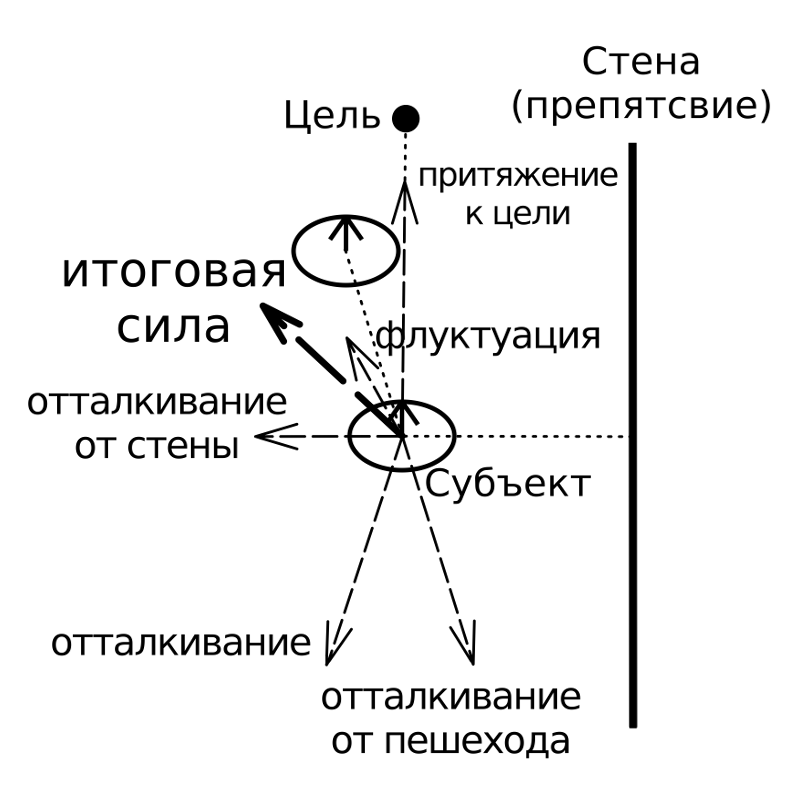
\includegraphics[width=\linewidth]{social_forces}
  \caption{Используемые социальные силы}
  \label{sec:model:sf:social_forces_pic}
\end{figure}

\subsubsection{Движущая сила в модели социальных сил}
\label{sec:model:sf:moving_force}

Движущая сила представляет побуждение пешехода достичь своей цели.
В случае, если цель не находится в прямой видимости, вводится последовательность промежуточных целей $\vec{r}_\alpha^k$.

Для полного описания движущей силы введем понятия желаемого направления и желаемой скорости.

Желаемое направление "--- вектор направления к следующей промежуточной цели, который определяется как:
\begin{equation}
  \label{sec:model:sf:moving_force:desired_direction_fm}
  \vec{e}_\alpha(t) = \vec{r}_\alpha^k - \vec{r}_\alpha(t)
\end{equation}
\begin{explanation}
где & $ \vec{r}_\alpha^k $ & вектор следующей промежуточной цели пешехода $\alpha$; \\
    & $ \vec{r}_\alpha(t) $ & текущая позиция пешехода $\alpha$ в момент времени $t$.
\end{explanation}

Желаемая скорость "--- скорость, с которой пешеход предпочел бы двигаться к цели.
В модели сделано предположение, что желаемая скорость пешеходов распределена нормально со средним значением в $1.34$ м/с и среднеквадратичным отклонением в $0.26$ м/с.

Также в оригинальной модели был введен вектор желаемой скорости $\vec{v}_\alpha^0(t)$
\begin{equation}
  \label{sec:model:sf:moving_force:desired_speed_fm}
  \vec{v}_\alpha^0(t) = v_\alpha^0(t) \vec{e}_\alpha(t)
\end{equation}
\begin{explanation}
где & $ v_\alpha^0 $ & желаемая скорость пешехода $\alpha$.
\end{explanation}

И выполнялась коррекция текущего направления движения с учетом времени релаксации (примерно $0.5$ с).
\begin{equation}
  \label{sec:model:sf:moving_force:force_fm}
  \vec{F}_\alpha^{moving}(t) = {{1}\over{t_\alpha}} ( \vec{v}_\alpha^0(t) - \vec{v}_\alpha(t) )
\end{equation}
\begin{explanation}
где & $ t_\alpha $ & время релаксации пешехода $\alpha$; \\
    & $ \vec{v}_\alpha(t) $ & текущая скорость пешехода $\alpha$ в момент времени $t$.
\end{explanation}

Таким образом, в оригинальной модели пешеход двигался не с желаемой скоростью в выбранном направлении, а с желаемой скоростью по направлению к цели.
В случае отсутствия каких-либо других социальных сил данное различие несущественно, однако оно может сильно исказить результаты при наличии социальных сил,
  имеющих схожее с движущей силой происхождение (например, при наличии силы объединения пешеходов в группы).

В связи с этим было принято решение выполнять коррекцию желаемой скорости не по одной движущей силе, а по сумме всех воздействующих сил.
Этим обеспечивается поддержание желаемой скорости вне зависимости от текущего направления движения.

\subsubsection{Отталкивающая сила в модели социальных сил}
\label{sec:model:sf:repulsion_force}

Сила отталкивания представляет побуждение пешехода сохранять некоторую дистанцию до других пешеходов и препятствий (стен).
Она направлена в противоположную от ближайшей точки препятствия сторону, а ее модуль в общем случае обратно зависит от расстояния до препятствия.
Авторы оригинальной модели социальных сил предлагают ввести поправочный коэффициент для учета анизотропности данной силы: пешеход держит большую дистанцию спереди и сзади, и меньшую – с боков.
Таким образом, модуль данной силы зависит не только от расстояния, но еще и от направления.

Отталкивающая сила между пешеходом $\alpha$ и препятсвием $\beta$ выражается как:
\begin{equation}
  \label{sec:model:sf:repulsion_force:force_fm}
  \vec{F}_{\alpha\beta}^{repulsion}(\vec{r}_{\alpha\beta}) = - \nabla V(r_{\alpha\beta})
\end{equation}
\begin{explanation}
где & $ r_{\alpha\beta} = r_\alpha - r_\beta $ & вектор направления от $\alpha$ к ближайшей точке $\beta$; \\
    & $ V(r_{\alpha\beta}) $ & функция, эквипотенциальные линии которой имеют форму эллипса.
\end{explanation}

\subsubsection{Учет поля зрения пешехода в модели социальных сил}
\label{sec:model:sf:fov}

Для большинства социальных сил имеет значение, мог ли данный пешеход видеть источник данной силы.
Для решения данной проблемы авторы оригинальной модели ввели еще один коэффициент, зависящий от угла между направлением движения и источником силы.
Данный коэффициент равен $1$, если угол между направлением движения и источником силы по модулю меньше некоторого заданного значения (в работе использовалось значение $100$ градусов), или $0.5$ в обратном случае.

Очевидным улучшением предложенной модели будет использование не дискретного порога, а некоторой непрерывной функции.

Для наглядности эту функцию можно представлять в виде некоторой формы на двумерной плоскости.
Интуитивно понятно, что данная форма представляет собой форму поля зрения пешехода.
Значение весовой функции определяется как длина вектора от центра координат к точке пересечения луча, проведенного из начала координат под соответствующим углом.

\begin{figure}[ht]
\centering
  \begin{subfigure}[b]{0.45\textwidth}
    \centering
    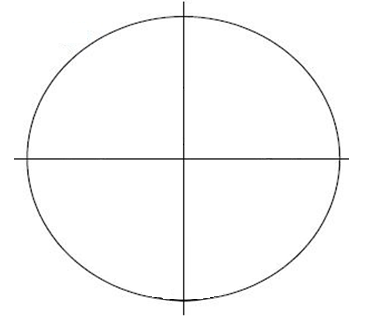
\includegraphics[scale=0.4]{fov_isotropic.png}
    \caption{}
  \end{subfigure}
  \begin{subfigure}[b]{0.45\textwidth}
    \centering
    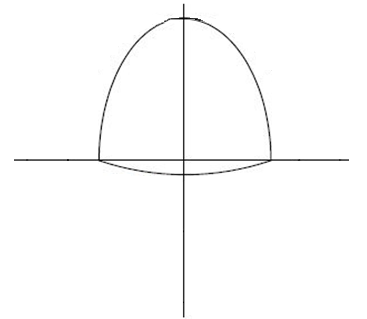
\includegraphics[scale=0.4]{fov_anisotropic.png}
    \caption{}
  \end{subfigure}
  \caption{ Примеры форм поля зрения пешехода: а "--- изотропная форма зрения;
            б "--- анизотропная форма зрения}
  \label{sec:model:sf:fov:example_figure}
\end{figure}

\subsubsection{Флуктуации в модели социальных сил}
\label{sec:model:sf:fluctuation}

Для более реалистичного поведения к итоговой сумме всех сил добавляются некоторые случайные флуктуации.
Основой флуктуаций с социальной точки зрения являются неучтенные мотивации или случайные импульсные решения пешехода.

Также добавление флуктуаций позволяет выходить из «тупиковых» ситуаций, когда сумма всех сил близка по модулю к нулю.

% не реализовано в ПС
\begin{comment}
\subsubsection{Моделирование паники с использованием модели социальных сил}
\label{sec:model:sf:panic}

Важным сценарием при тестировании является сценарий паники. В данном случае поведение пешеходных потоков значительно меняется и требует других средств и методов моделирования.

На основе изучения различных социальных исследований, выделяют следующие отличия в поведении людей при панике \cite{helbing_panic}:
\begin{itemize}
  \item люди двигаются (или пытаются двигаться) значительно быстрее чем обычно;
  \item люди перестают поддерживать безопасное личное расстояние и начинают взаимодействовать физически;
  \item люди начинают проявлять склонность к массовому поведению (повторять поведение окружающих людей).
\end{itemize}

Для того, чтобы учесть данные отличия, введем в модель некоторые переменные.

Первой переменной, необходимой для моделирования сценария паники, является уровень паники.
Источниками паники являются какие-либо опасные объекты.
Также уровень паники может распространятся по близко стоящим друг к другу людям.
Определим уровень паники как
\begin{equation}
  \label{sec:model:sf:panic:level}
  ppl_\alpha = kspl \sum\limits_{i=1}^n {{ppl_i}\over{||\vec{r}_\alpha - \vec{r}_i||}} + kdpl \sum\limits_{i=1}^m {{spl_i}\over{||\vec{r}_\alpha - \vec{r}_i||}}
\end{equation}
\begin{explanation}
где & $ kspl $ & коэффициент распространения паники; \\
    & $ kdpl $ & коэффициент начального приобретения паники; \\
    & $ ppl_i $ & уровень паники $i$-ого пешехода; \\
    & $ spl_i $ & уровень паники $i$-ого опасного объекта; \\
    & $ n $ & количество других пешеходов в поле зрения пешехода; \\
    & $ m $ & количество опасных объектов в поле зрения пешехода; \\
    & $ ||\vec{r}_\alpha - \vec{r}_i|| $ & расстояние от пешехода $\alpha$ до источника паники $i$.
\end{explanation}

Также следует отметить важность выбора коэффициента распространения паники $kspl$.
Если установить для данного значения слишком низкое значение, то эффект лавинообразного возникновения паники не появится.
Если же установить слишком высокое значение, то пешеходы могут войти в состояние паники даже от незначительных воздействий.

Желаемая скорость с учетом паники определяется как

\begin{equation}
  \label{sec:model:sf:panic:desired_speed}
  vpanic_\alpha^0 = kspeedpl \cdot ppl_\alpha v_\alpha^0
\end{equation}
\begin{explanation}
где & $ kspeedpl $ & коэффициент учета паники в желаемой скорости.
\end{explanation}

А отталкивающая сила определяется как

\begin{equation}
  \label{sec:model:sf:panic:repulsion_force}
  \vec{Fpanic}_{\alpha\beta}^{repulsion}(\vec{r}_{\alpha\beta}) = krepulsionpl {{1}\over{ppl_\alpha ppl_\beta}}\vec{F}_{\alpha\beta}^{repulsion}(\vec{r}_{\alpha\beta})
\end{equation}
\begin{explanation}
где & $ kspeedpl $ & коэффициент учета паники в силе отталкивания.
\end{explanation}

Также люди начинают копировать желаемое направление окружающих людей. Этот эффект можно описать как

\begin{equation}
  \label{sec:model:sf:moving_force:desired_direction_fm}
  \vec{epanic}_\alpha(t) = kdirectionpl \cdot ppl_\alpha \sum\limits_{i=1}^n \vec{e}_\alpha(t)
\end{equation}
\begin{explanation}
где & $ kdirectionpl $ & коэффициент учета паники в желаемом направлении; \\
    & $ n $ & количество других пешеходов в поле зрения пешехода.
\end{explanation}

\subsection{Функциональная спецификация разрабатываемого ПС}
\label{sec:model:func_spec}

В результате анализа предметной области и разработки собственной модификации модели социальных сил, к разрабатываемому ПС были выдвинуты следующие функциональные требования:
\begin{itemize}
  \item Разрабатываемое ПС должно выполнять симуляцию пещеходных потоков по модели социальных сил.
        Входными данными являются сценарий симуляции и план помещения, а выходными "--- либо файл с результатами моделирования в унифицированном формате, либо 2D анимация с отмеченными вероятными местами скопления людей.
        План помещения задается в формате SVG, где значимым с точки зрения симуляции объектам проставлены определенные атрибуты.
        Все используемые форматы (формат сценария симуляции, формат результатов моделирования, формат плана помещения) должны быть полностью описаны в документации.
  \item Разрабатываемое ПС должно позволять выполнять как симуляцию в режиме реального времени, так и воспроизведение заранее сгенерированного файла результатов симуляции.
  \item Гибкая настройка модели и сценария симуляции.
        Большинство значимых параметров модели и сценария должны быть изменяемыми из файла описания сценария симуляции.
  \item Наличие возможности интеграции моделирования в существующее приложение.
        Сторонние приложения могут импортировать результаты симуляции и выполнять над ними определенные действия.
  \item Высокая скорость работы.
        Разрабатываемое приложение должно обеспечивать возможность просмотра результатов симуляции в режиме реального времени для как минимум одной сотни пешеходов.
\end{itemize}
\end{comment}


\section{Проектирование программного средства} % (fold)
\label{sec:development}

Разрабатываемым программное средство, как было отмечено в пункте~\ref{sub:domain:requirements:langs}, было разбито на три независимых модуля.
Каждый модуль разрабатывался отдельно. Модули обмениваются данными в определенном бинарном формате.
Это позволяет сторонним приложениям легко интегрироваться с разрабатываемым ПС путем реализации чтения описанных ниже бинарных форматов.

Диаграмма потоков данных изображена на рисунке~\ref{sec:development:data_flow_diagramm}, а общая схема работы ПС "--- на рисунке~\ref{sec:development:general_working_scheme}.

\begin{figure}[ht]
  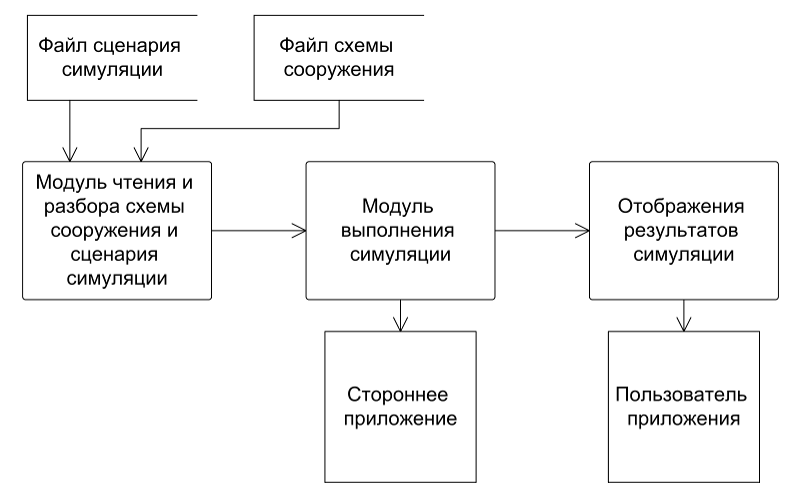
\includegraphics[width=\linewidth]{dfd}
  \caption{Диаграмма потоков данных}
  \label{sec:development:data_flow_diagramm}
\end{figure}

\begin{figure}[!ht]
  \centering
  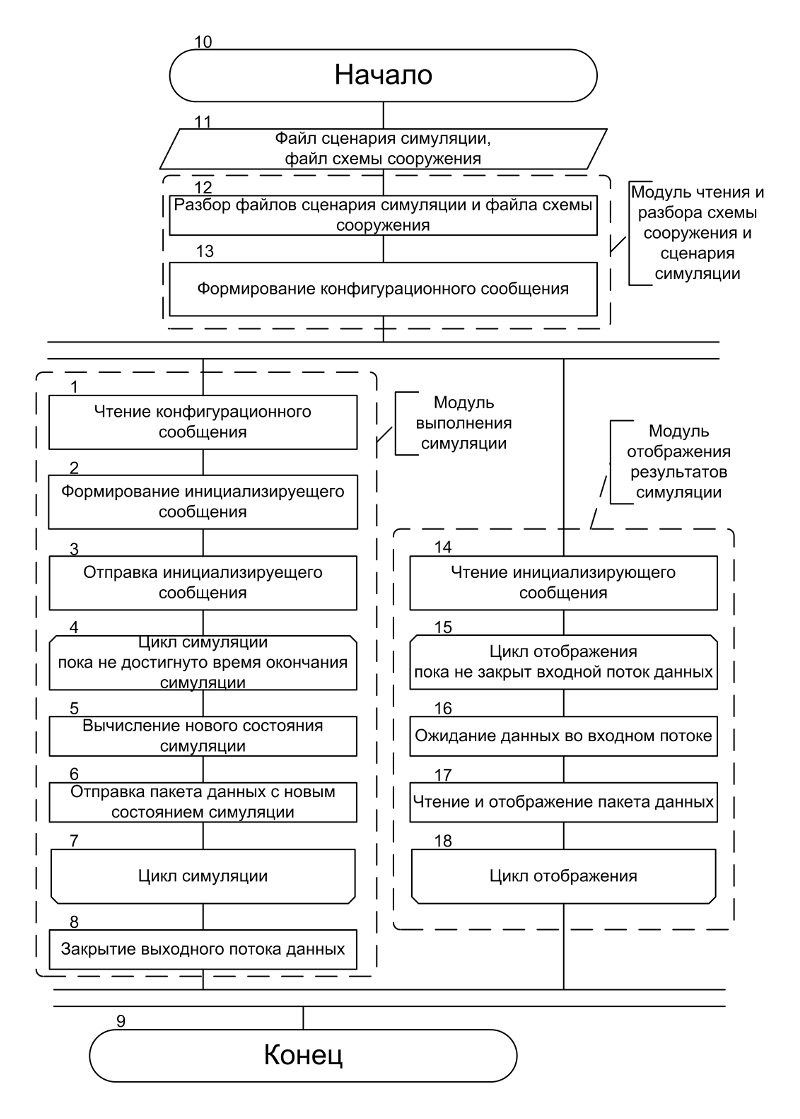
\includegraphics[width=\dimexpr\linewidth-10em\relax]{general_working_scheme}
  \caption{Схема работы системы определения вероятных областей скопления}
  \label{sec:development:general_working_scheme}
\end{figure}

В данном разделе будут подробно рассмотрены все модули, используемые в разрабатываемом ПС, а также будут описаны бинарные форматы обмена данными.

\subsection{Модуль чтения и разбора схемы сооружения и сценария симуляции}
\label{sec:development:preprocessor}

Модуль чтения и разбора схемы сооружения и сценария симуляции выполнен на языке программирования Ruby~\cite{ruby_doc}.
В его задачи входит:
\begin{itemize}
  \item разбор сценария симуляции на отдельные компоненты;
  \item разбор схемы сооружения на отдельные компоненты;
  \item формирование сообщения о конфигурации модулю выполнения симуляции в определенном бинарном формате.
\end{itemize}

\subsubsection{Сценарий симуляции}
\label{sec:development:preprocessor:scenario_dsl}

Благодаря гибкости языка Ruby и его широких возможностей в метапрограммировании,
сценарий симуляции выполнен в виде предметно"=ориентированного языка (DSL "--- Domain Specific Language).

Пример сценария симуляции представлен в листинге~\ref{sec:development:preprocessor:scenario_dsl_listing}.

\lstinputlisting[language=Ruby,basicstyle=\small,caption={Пример сценария симуляции}, label=sec:development:preprocessor:scenario_dsl_listing, texcl=true]{sim_params_example.rb}

В сценарии симуляции указывается множество различных параметров симуляции.
Более подробно данный язык и каждый его параметр будут рассмотрены в разделе~\ref{sec:manual:input:scenario}.
В данном разделе остановимся на рассмотрении вопросов, связанных с реализацией данного предметно"=ориентированного языка.

Основой разработанного модуля является класс Sections::Base. Он представляет собой базовый класс для определения секции в файле сценария симуляции.
Данный класс определяет статический метод field, который добавляет во внутренние переменные класса предоставленную информацию о поле сценария симуляции,
а также средствами метапрограммирования Ruby (в частности, с помощью метода define\_method) объявляет в вызывающем классе метод с именем, соответствующим имени поля.
Данный метод при вызове получает некоторое значение поля и сохраняет его во внутренней переменной объекта класса.
Таким образом, файл сценария симуляции по сути является файлом с Ruby кодом, который вызывает объявленные ранее методы с именами полей.

Поддерживаются следующие типы полей: целое число, число с плавающей точкой, строка, булевый флаг, потомок, распределение и динамический тип.

Потомок "--- особый тип поля, которому в параметрах передается имя класса, отвечающего за дальнейший разбор предоставленных параметров.
Данный тип поля использует такую особенность языка Ruby, как блоки, которые являются реализацией общей концепции замыканий.
В языке Ruby существует четыре концепции, описывающие некоторую совокупность кода "--- это block, Proc, lambda и method.

Proc "--- объект, описывает некоторую абстрактную совокупность кода. Он может быть сохранен в отдельную переменную. Доступ к коду, который хранит Proc, осуществляется с помощью метода call(args).
Lambda по своей сути практически не отличается от объекта Proc. Отличиями являются наличие контроля за передаваемыми аргументами и другое поведение оператора return внутри хранимого кода.
Method "--- объект-обертка над lambda. Используется для хранения методов внутри класса. Так же как Proc и lambda, использует метод call(args) для доступа к коду.

Блоки в руби являются своеобразным синтаксическим сахаром над описанными выше концепциями.
Они позволяют унифицировать доступ к определенным совокупностям кода с помощью единого синтаксиса.
В частности, любой метод в руби может принимать дополнительный последний параметр, отмеченный специальным символом \&.
В случае, если метод был вызван с блоком, в данный параметр передается сконвертированная в объект Proc совокупность кода, находящаяся в блоке.
Так же в Ruby присутствует функция yield, которая вызывает код, переданный в блоке, с определенными параметрами.

Таким образом, поле типа <<потомок>> принимает на вход блок, и выполняет его содержимое в контексте определенного класса-потомка.

Распределение "--- еще один особый тип поля. Он очень похож на <<потомка>>, за исключением того, что переданный блок всегда выполняется в контексте определенного класса (Utils::Distribution),
который отвечает за формирование определенных полей в зависимости от типа распределения (равномерное, нормальное и др.).

Последний тип поля "--- динамический тип. Он позволяет обрабатывающему классу определить некоторую совокупность кода, которая будет осуществлять разбор предоставленного значения.
В качестве совокупности кода может выступать любая из четырех описанных выше концепций.

\subsubsection{Схема сооружения}
\label{sec:development:preprocessor:svg_scheme}

В качестве схемы сооружения используется особым образом модифицированный SVG файл.
SVG~\cite{svg_home} "--- распространенный формат векторной графики на основе XML.
Выбор SVG в качестве формата для представления схемы сооружения обусловлен следующими причинами:
\begin{itemize}
  \item распространенность формата SVG;
  \item легкость модификации SVG элементов путем добавления атрибутов к соответствующим XML тегам;
  \item легкость разбора SVG файлов на компоненты.
\end{itemize}

Пример схемы сооружения представлен в листинге~\ref{sec:development:preprocessor:svg_scheme_listing}.

\lstinputlisting[language=XML,basicstyle=\small,caption={Пример схемы сооружения}, label=sec:development:preprocessor:svg_scheme_listing]{scene.svg}

В реализованном ПС поддерживаются два основных элемента SVG "--- line и rect.
При этом введены следующие дополнительные атрибуты:
\begin{itemize}
  \item x-csim-class;
  \item x-csim-id;
  \item x-csim-seq-no;
  \item x-csim-last.
\end{itemize}

Атрибут x-csim-class отвечает за тип данного элемента.
Возможные значения:
  wall (препятствие),
  spawn\_area (место появления людей),
  target\_area (место назначения людей "--- промежуточное или конечное).

Атрибут x-csim-id отвечает за идентификацию определенного логического элемента.
В частности, он используется для связывания цепочки мест появления и мест назначения в единый путь.

Атрибут x-csim-seq-no может быть применен только к элементу с типом target\_area и определяет порядковый номер промежуточной target\_area.

Атрибут x-csim-last определяет, является ли данное место назначения промежуточным или конечным.

Поле, задающее путь к файлу со схемой сооружения в сценарии симуляции, имеет динамический тип.
В качестве обработчика указан метод класса Sections::Scene parse\_scene\_file.
Данный метод осуществляет разбор схемы сооружения с использованием библиотеки разбора XML Crack~\cite{ruby_crack_gem}, и сохраняет полученные геометрические элементы с их признаками.

\subsubsection{Формирование сообщения о конфигурации модулю выполнения симуляции}
\label{sec:development:preprocessor:format}

После разбора всех компонентов сценария симуляции модуль чтения и разбора должен сформировать сообщение о конфигурации модулю выполнения симуляции.
Для выполнения данной задачи каждый класс, представляющий собой секцию в файле конфигурации, обязан предоставить метод to\_config, который сформирует бинарную строку по определенному формату.
Данный метод вызывается рекурсивно для всех потомков, что позволяет на вершине дерева собрать все необходимое сообщение о конфигурации.

Формат описания конфигурации состоит из отдельных независимых друг от друга элементов.
Каждый элемент имеет следующую структуру:
\begin{itemize}
  \item идентификатор секции, к которой принадлежит данный элемент (1 байт);
  \item идентификатор элемента внутри данной секции (2 байта);
  \item данные элемента, закодированные в бинарном формате (переменное количество байт).
\end{itemize}

Подробно данные каждого элемента описаны в таблице~\ref{sec:development:preprocessor:format_table}.
Все координаты представлены двухбайтовыми целыми числами без знака, а перед каждой строкой записана ее длина.
Также используется формат распределения, который во всех случаях состоит из одного однобайтового целого без знака и двух чисел с плавающей точкой.
Первое число определяет тип распределения "--- равномерное (0x01) или нормальное (0x02).
В случае равномерного два числа с плавающей точкой означают границы <<от>> и <<до>> распределения,
а в случае нормального "--- среднее значение и среднеквадратичное отклонение соответственно.

\newpage
\begin{longtable}[ht]{| >{\centering}m{0.25\textwidth}
                      | >{\centering}m{0.25\textwidth}
                      | >{\centering\arraybackslash}m{0.40\textwidth}|}
\caption{Формат сообщения о конфигурации} \label{sec:development:preprocessor:format_table}\tabularnewline

\hline Секция & Элемент & Данные элемента \tabularnewline
\endfirsthead
\captionsetup{labelformat=stbtablecont,justification=raggedright}
\caption[]{}\tabularnewline
\hline 1 & 2 & 3 \tabularnewline
\endhead
  \hline Сцена "--- 0x01 & Стена (препятствие) "--- 0x0001 & \specialcell{координаты первой точки\\
                                                                       (x0, y0)\\
                                                                       координаты второй точки\\
                                                                       (x1, y1)} \tabularnewline
  \hline Сцена "--- 0x01 & Место появления людей "--- 0x0002 & \specialcell{координаты первой точки\\
                                                                           (x0, y0)\\
                                                                           координаты второй точки\\
                                                                           (x1, y1)\\
                                                                           идентификатор пути (1 байт)} \tabularnewline
  \hline Сцена "--- 0x01 & Место назначения "--- 0x0003 & \specialcell{координаты первой точки\\
                                                                       (x0, y0)\\
                                                                       координаты второй точки\\
                                                                       (x1, y1)\\
                                                                       идентификатор пути\\
                                                                       (целое, 1 байт)\\
                                                                       порядковый номер\\
                                                                       (целое, 7 бит)\\
                                                                       флаг конечности (1 бит)} \tabularnewline
  \hline Сцена "--- 0x01 & Ширина, пикселей "--- 0x0011 & ширина (целое, 2 байта) \tabularnewline
  \hline Сцена "--- 0x01 & Высота, пикселей "--- 0x0012 & высота (целое, 2 байта) \tabularnewline
  \hline Сцена "--- 0x01 & Масштаб, метров на пиксель "--- 0x0013 & масштаб (с плавающей точкой, 8 байт) \tabularnewline
  \hline Сцена "--- 0x01 & Имя файла со сценой "--- 0x00FF & имя файла (строка) \tabularnewline

  \hline Параметры времени "--- 0x02 & Время окончания симуляции, секунд "--- 0x0001 & время (целое, 4 байта) \tabularnewline
  \hline Параметры времени "--- 0x02 & Единичный шаг времени, секунд "--- 0x0002 & шаг (с плавающей точкой, 8 байт) \tabularnewline

  \hline Параметры места появления "--- 0x03 & Скорость появления, человек в секунду "--- 0x0001 & скорость (с плавающей точкой, 8 байт) \tabularnewline

  \hline Параметры сил "--- 0x04 & Коэффициент отталкивания "--- 0x0101 & коэффициент (распределение) \tabularnewline
  \hline Параметры сил "--- 0x04 & Желаемая скорость передвижения "--- 0x0201 & скорость (распределение) \tabularnewline

  \hline Параметры поля зрения "--- 0x05 & Коэффициент переднего поля зрения "--- 0x0001 & коэффициент (распределение) \tabularnewline
  \hline Параметры поля зрения "--- 0x05 & Коэффициент заднего поля зрения "--- 0x0002 & коэффициент (распределение) \tabularnewline

  \hline Параметры определения плотности "--- 0x06 & Флаг включения "--- 0x0001 & \specialcell{флаг (1 байт)\\
                                                                                               1 "--- включено\\
                                                                                               0 "--- выключено} \tabularnewline
  \hline Параметры определения плотности "--- 0x06 & Минимальный порог плотности (ниже данного порога область не считается областью скопления) "--- 0x0002 & порог (с плавающей точкой, 8 байт) \tabularnewline
  \hline Параметры определения плотности "--- 0x06 & Максимальный порог плотности (выше данного порога области не различаются между собой по цвету) "--- 0x0003 & порог (с плавающей точкой, 8 байт) \tabularnewline

  \hline
\end{longtable}

\subsection{Модуль выполнения симуляции}
\label{sec:development:core}

Модуль выполнения симуляции разработан на языке программирования Rust~\cite{rust_doc}.
В его задачи входит:
\begin{itemize}
  \item разбор и сохранение входного сообщения о конфигурации;
  \item выполнение симуляции по заданной конфигурации;
  \item в процессе выполнения непрерывно выдавать данные о текущем состоянии симуляции модулю отображения результатов.
\end{itemize}

\subsubsection{Разбор и сохранение конфигурации}
\label{sec:development:core:configuration}

Разбор и сохранение конфигурации осуществляется подмодулем con\-fi\-gu\-ra\-ti\-on.
Экспортируемыми элементами из данного модуля являются
функция new, которая осуществляет разбор предоставленной конфигурации и сохранение ее в новое хранилище,
макрос config, который получает значение определенного параметра из хранилища,
а также множество типов (структур и перечислений), используемых в качестве ключей для доступа к конфигурации.

В качестве хранилища для конфигурации была выбрана библиотека AnyMap~\cite{rust_anymap_cargo}.
Данная библиотека позволяет хранить по ключу в виде типа некоторое значение данного типа.
Соответственно, в модуле configuration объявлено по одному типу на каждый элемент конфигурации.

Основной цикл разбора конфигурации находится в функции par\-se\_con\-fig\_fi\-le.
Данная функция вызывает функцию par\-se\_sin\-gle\_item до тех пор, пока не останется ни одного необработанного элемента.

Функция parse\_single\_item читает из входного потока номер секции, и в зависимости от него вызывает одну из функций
par\-se\_sce\-ne\_item (секция сцены), par\-se\_time\_item (секция параметров времени),
par\-se\_spawn\_item (секция параметров мест появления),
par\-se\_for\-ces\_item (секция параметров социальных сил),
par\-se\_fov\_item (секция параметров поля зрения)
или par\-se\_den\-si\-ty\_map\_item (секция параметров плотностей потоков).
Каждая из этих функций читает из входного потока номер элемента конфигурации,
а потом в зависимости от элемента читает нужное количество параметров с помощью функций чтения элементарных типов.

В качестве функций чтения элементарных типов в модуле configuration реализованы:
par\-se\_u8 (чтение однобайтового беззнакового целого числа),
par\-se\_u16 (чтение двухбайтового беззнакового целого числа),
par\-se\_u32 (чтение четырехбайтового беззнакового целого числа),
par\-se\_f64 (чтение восьмибайтового числа с плавающей точкой),
par\-se\_string (чтение строки),
par\-se\_co\-or\-di\-na\-tes (чтение набора из четырех координат),
par\-se\_dis\-tri\-bu\-ti\-on (чтение элемента распределения).

\subsubsection{Выполнение симуляции}
\label{sec:development:core:simulation}

Выполнение симуляции осуществляется модулем si\-mu\-la\-ti\-on.
Вначале происходит инициализация процесса, при которой все подмодули симуляции получают нужные значения из конфигурации.

В модуле simulation объявлено два основных метода "--- main\_loop и update\_state.

Метод main\_loop в цикле выполняет следующие действия:
\begin{itemize}
  \item обновить состояние (update\_state);
  \item сформировать сообщений о текущем состоянии;
  \item передвинуть время симуляции на следующий шаг;
  \item повторять пока не достигнуто время конца симуляции.
\end{itemize}

Метод update\_state служит для обновления состояния симуляции и выполняет следующие действия:
\begin{itemize}
  \item рассчитывает итоговую силу для каждого пешехода;
  \item сдвигает каждого пешехода в соответствии с рассчитанной итоговой силой;
  \item создает новых пешеходов в областях появления;
  \item обрабатывает пешеходов, достигших своей точки назначения.
\end{itemize}

Для выполнения своих целей модуль симуляции использует следующие подмодули:
\begin{itemize}
  \item person;
  \item time;
  \item forces;
  \item scene.
\end{itemize}

Подмодуль person отвечает за представление одного пешехода.
Для каждого пешехода хранится следующая информация:
\begin{itemize}
  \item координаты пешехода;
  \item направление пешехода;
  \item идентификатор пути в сцене, по которому движется пешеход;
  \item текущая цель пешехода;
  \item структура, которая хранит параметры сил, характерные для данного пешехода (желаемая скорость, коэффициент отталкивания).
\end{itemize}

Основным методом, объявленным на классе Person, является метод перемещения под воздействием силы (move\_by).
Данный метод принимает результирующую силу, воздействующую на пешехода, и время.
Пешеход сдвигается на соответствующее расстояние, и новым направлением для него становится направление силы.

Также у класса Person есть вспомогательный метод reached\_destination, который определяет, достиг ли пешеход своей текущей цели.

Подмодуль time отвечает за управление временем симуляции и хранит текущее время, время окончания и время одного шага.
В нем объявлены следующие методы:
\begin{itemize}
  \item is\_passed "--- возвращает истину в случае, если достигнуто время окончания (симуляция закончена);
  \item next\_tick "--- переводит время симуляции на один шаг вперед.
\end{itemize}

Подмодуль forces отвечает за используемые при симуляции силы.
Он экспортирует два основных метода "--- расчет результирующей социальной силы (total\_force\_for\_person)
и метод генерации структуры параметров сил для нового пешехода (generate\_person\_forces\_param).

Схема программы расчета результирующей социальной силы представлена на рисунке~\ref{sec:development:core:total_force_calc_pic}.

\begin{figure}[!ht]
  \centering
  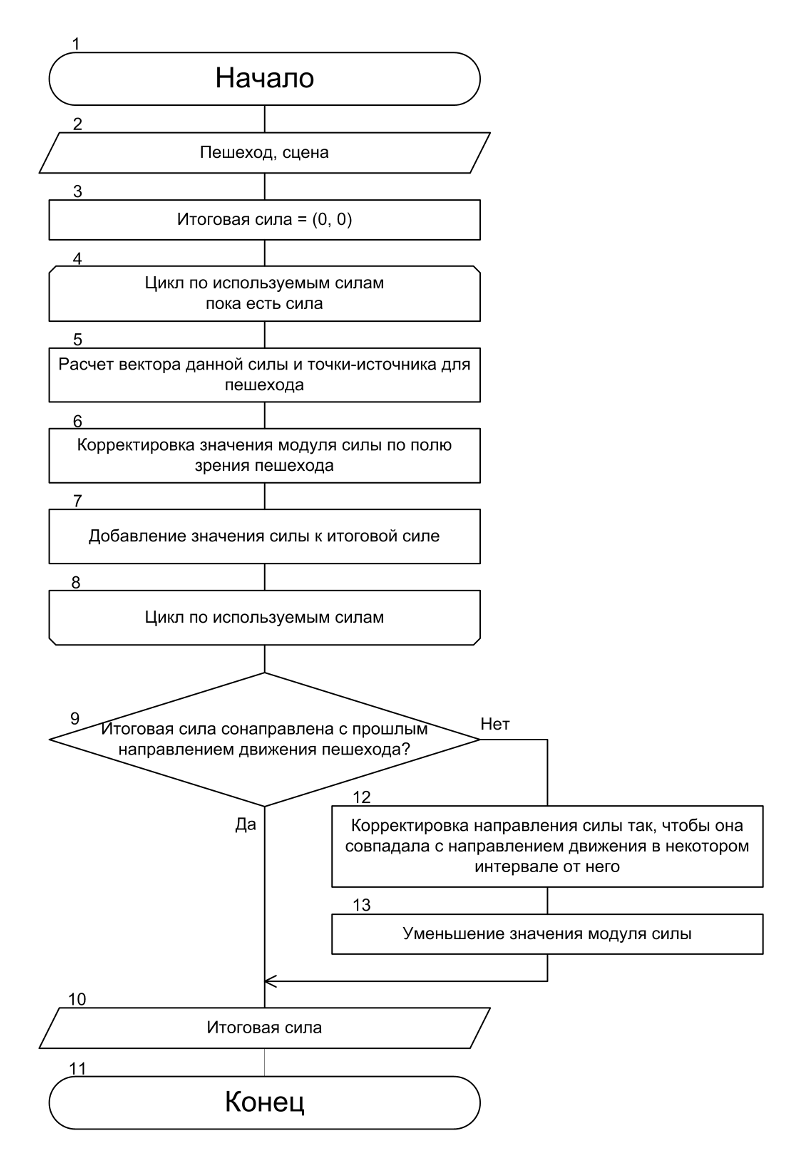
\includegraphics[width=\dimexpr\linewidth-10em\relax]{total_force_scheme}
  \caption{Схема программы расчета результирующей социальной силы}
  \label{sec:development:core:total_force_calc_pic}
\end{figure}

Как видно из представленной схемы программы, данный метод использует аналог интерфейса (в языке Rust они называются traits) для получения значения каждой используемой социальной силы.
В данном интерфейсе определено, что сила получает на вход пешехода и сцену, и должна вернуть некоторый вектор воздействия на пешехода, а также точку источника силы.
Также стоит отметить, что для хранения всех используемых социальных сил используется единое перечисление.

После определения всех социальных сил, воздействующих на пешехода, осуществляется коррекция по полю зрения.
Для этого вектор каждой силы домножается на коэффициент, зависящий от формы поля зрения пешехода и направления к источнику силы.

После суммирования всех скорректированных социальных сил, воздействующих на пешехода, проверяется, повернут ли пешеход в нужную сторону (в сторону результирующей силы).
Если же пешеход не повернут в нужную сторону, то происходит перерасчет новой силы поворота (которая не так сильно отличается от исходного направления пешехода) с ограниченным модулем.
Таким образом, пешеход не может мгновенно развернуться, что добавляет модели реалистичности.

Последним подмодулем является scene.
Он является контейнером для всех объектов моделирования (пешеходов, препятствий, путей следования).
Для большинства объектов моделирования в качестве примитива хранения выбран вектор (абстракция над массивом динамической длины в куче).
Это обусловлено тем, что большинство объектов на сцене статичны и не меняются.
Однако данное утверждение не справедливо для пешеходов, в связи с чем для их хранения используется другой примитив "---
двусвязный список с использованием его реализации LinkedList~\cite{rust_linked_list_cargo}. Это позволяет быстро удалять пешеходов из середины списка.

Важными экспортируемыми методами модуля scene являются spa\-wn\_peo\-ple, pro\-cess\_reach\-ed\_des\-ti\-na\-ti\-on\_people, и get\_den\-si\-ty\_map.

Метод spawn\_people отвечает за создание новых пешеходов в областях появления пешеходов.
Сначала метод выбирает свободное место для пешехода внутри области появления.
Для этого он некоторое конечное число раз пытается случайно сгенерировать координаты внутри данной области.
Если все сгенерированные координаты были заняты, то в системный лог пишется предупреждение о том, что область появления переполнена.
Если же место для пешехода нашлось, то создается новый объект класса Person.

Метод process\_reached\_destination\_people отвечает за следование пешеходами вдоль их пути.
Данный метод выбирает тех пешеходов, которые достигли своей текущей цели.
Далее производится проверка, была ли достигнутая пешеходом цель, которая является последней в цепочке.
Если да, то данный пешеход удаляется как достигший своей цели. Если нет, то в качестве текущей цели пешеходу проставляется следующая по цепочке цель.

Метод get\_density\_map отвечает за расчет карты плотностей пешеходных потоков.
Он использует следующий алгоритм определения плотности в каждой точке сцены:
\begin{itemize}
  \item инициализировать двумерный массив плотностей нулями;
  \item для каждого пешехода внутри сцены:
  \item для каждой точки на некотором расстоянии от пешехода:
  \item добавить в данную точку значение плотности, зависящее от расстояния до пешехода.
\end{itemize}

В качестве зависимости плотности от расстояния до пешехода выбрана аппроксимация гауссового распределения.
Таким образом, мы получаем непрерывную плавную карту плотностей пешеходных потоков внутри сцены.

\subsubsection{Вспомогательные подмодули, используемые при симуляции}
\label{sec:development:core:utils}

При выполнении симуляции использовались некоторые вспомогательные подмодули в составе модуля utils.

Первым таким подмодулем является подмодуль linelg "--- реализация линейной алгебры~\cite{linelg_book}.
В нем реализованы структуры данных и операции над такими сущностями, как точка, вектор, линия, расстояние и др.
При разработке данного модуля широко использовались возможности языка Rust по перегрузке операторов,
что позволило сделать код, использующий данный модуль, более лаконичным.

Вторым подмодулем является distributions "--- реализация генерирования значения случайной величины, описанной определенной структурой.
Генерирование значения для равномерного распределения осуществляется методом обратной функции,
а для нормального распределения "--- методом на основе центральной предельной теоремы~\cite{probability_modeling}.

\subsubsection{Формирование сообщений о текущем состоянии симуляции модулю отображения результатов}
\label{sec:development:core:output}

За формирование сообщений о текущем состоянии симуляции отвечает подмодуль output.
Так же как и модуль simulation, при инициализации он принимает объект конфигурации, из которого он получает нужные ему элементы.

Формат сообщений модулю отображения результатов можно разбить на два отдельных сообщения: инициализирующее сообщение и сообщение о текущем состоянии.

Посылку инициализирующего сообщения осуществляет метод se\-nd\_in\-it.
В составе инициализирующего сообщения посылается информация в следующем порядке:
\begin{itemize}
  \item длина строки с именем svg файла схемы сооружения (беззнаковое число, 2 байта);
  \item строка с именем svg файла схемы сооружения;
  \item масштаб svg файла схемы сооружения, метров на пиксель (число с плавающей точкой, 8 байт);
  \item флаг наличия карт плотности пешеходных потоков: 1 "--- есть, 0 "--- нету (беззнаковое число, 1 байт);
  \item минимальная плотность пешеходных потоков (число с плавающей точкой, 8 байт);
  \item максимальная плотность пешеходных потоков (число с плавающей точкой, 8 байт).
\end{itemize}

После этого на каждом такте осуществляется посылка сообщения о текущем состоянии с помощью метода dump\_state.
Каждое сообщение о текущем состоянии состоит из следующих полей:
\begin{itemize}
  \item текущее время симуляции (число с плавающей точкой, 8 байт);
  \item в случае, если карты плотности пешеходных потоков включены: флаг наличия в данном сообщении информации о плотности пешеходных потоков (беззнаковое число, 1 байт);
  \item в случае, если флаг наличия информации о плотности пешеходных потоков установлен: количество точек с плотностью выше минимальной (беззнаковое число, 4 байта);
  \item в случае, если флаг наличия информации о плотности пешеходных потоков установлен: массив из точек с повышенной плотностью в формате
    координата по горизонтали (беззнаковое число, 2 байта), координата по вертикали (беззнаковое число, 2 байта), плотность (число с плавающей точкой, 8 байт);
  \item количество пешеходов (беззнаковое число, 4 байта);
  \item массив из координат пешеходов и их направлений в формате
    координата по горизонтали (беззнаковое число, 2 байта), координата по вертикали (беззнаковое число, 2 байта), направление (число с плавающей точкой, 8 байт).
\end{itemize}

Важным моментом является опциональное присутствие карты плотности в сообщении.
Это обусловлено тем, что расчет карты плотности достаточно трудоемкая задача, и делать данный расчет на каждой итерации симуляции не имеет смысла.
Вместо этого, расчет карты плотности производится каждую секунду модельного времени.

Также стоит упомянуть, что направление представляет собой угол от положительного направления оси абсцисс в радианах и имеет область значений от $0$ до $2\pi$.

\subsection{Модуль отображения результатов симуляции}
\label{sec:development:animator}

Модуль отображения результатов симуляции выполнен на языке программирования С с использованием библиотеки SDL~\cite{libsdl_home}.
В его задачи входит:
\begin{itemize}
  \item реализация ожидания следующего состояния в случае, если модуль выполнения симуляции не успевает слать данные в режиме реального времени;
  \item разбор данных о текущем состоянии симуляции;
  \item отображение текущего состояния симуляции на экране.
\end{itemize}

\subsubsection{Реализация ожидания следующего состояния симуляции}
\label{sec:development:animator:wait}

В качестве реализации ожидания следующего состояния был выбран системный вызов select,
который позволяет заблокировать текущий поток на определенное время (или на неограниченное время),
до тех пор пока переданные ему файловые дескрипторы не станут доступны для чтения, записи либо чтения ошибки.

Таким образом, перед началом каждого цикла считывания текущего состояния реализуемый модуль вызывает функцию select с дескриптором на чтение и засыпает до тех пор,
пока от модуля выполнения симуляции не придут данные.

\subsubsection{Разбор данных о текущем состоянии симуляции}
\label{sec:development:animator:parse}

По причине простоты формата сообщения о текущем состоянии симуляции, операции по их разбору не вынесены в отдельный подмодуль и осуществляются прямо в главном цикле данного модуля.
Для осуществления чтения элементарных типов в контроллере объявлены следующие методы:
\begin{itemize}
  \item unsigned char controller\_read\_byte();
  \item unsigned short controller\_read\_short();
  \item unsigned long controller\_read\_long();
  \item char* controller\_read\_string();
  \item double controller\_read\_double().
\end{itemize}

\subsubsection{Отображение текущего состояния симуляции на экране}
\label{sec:development:animator:show}

Схема программы отображения результатов расчета изображена на рисунке~\ref{sec:development:animator:main_cycle_pic}.

\begin{figure}[!ht]
  \centering
  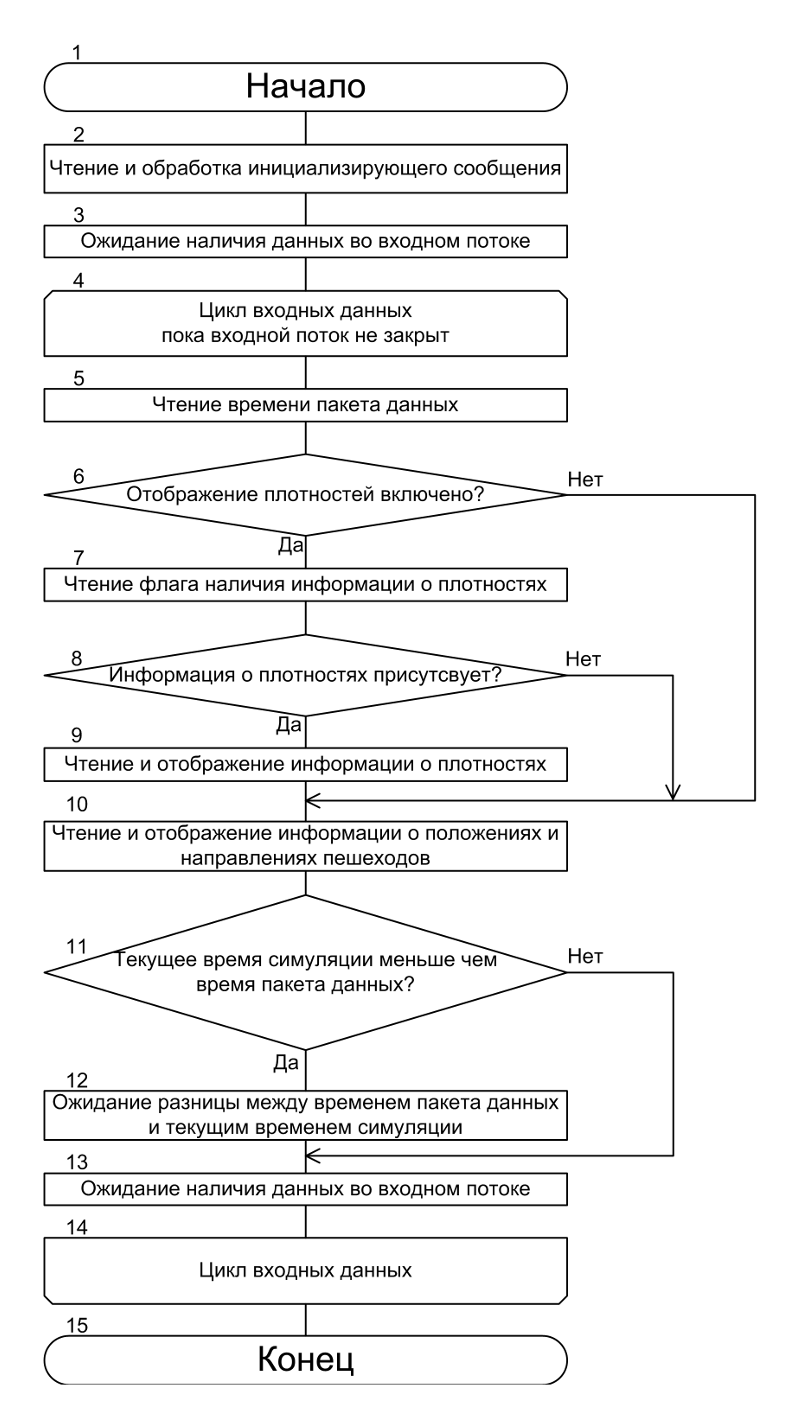
\includegraphics[width=\dimexpr\linewidth-10em\relax]{animator_scheme}
  \caption{Схема программы отображения результатов расчета}
  \label{sec:development:animator:main_cycle_pic}
\end{figure}

Как можно заметить на приведенной схеме, последовательность действий модуля отображения текущего состояния симуляции следующая:
\begin{itemize}
  \item проинициализировать все системы библиотеки SDL;
  \item прочитать инициализационное сообщение от модуля выполнения симуляции;
  \item загрузить и подготовить все необходимые текстуры из SVG файлов;
  \item войти в главный цикл;
  \item осуществить очистку всех используемых ресурсов.
\end{itemize}

При этом в главном цикле выполняются следующие задачи:
\begin{itemize}
  \item ожидать сообщения о следующем состоянии симуляции от модуля выполнения симуляции;
  \item прочитать время симуляции пакета данных;
  \item очистить экран;
  \item вывести на экран текстуру со сценой;
  \item если присутствует информация о плотностях: прочитать данную информацию, сформировать и отобразить текстуру с плотностями;
  \item прочитать и отобразить информацию о пешеходах;
  \item рассчитать текущее время симуляции как разницу между текущим временем и временем начала симуляции;
  \item если текущее время симуляции меньше чем время пакета данных, ожидать нужное количество времени;
  \item обновить экран новыми данными.
\end{itemize}

Загрузка и растеризация SVG файлов осуществлялась с помощью библиотек librsvg~\cite{librsvg_home} и cairo~\cite{cairo_home}.

Все описанные выше задачи достаточно просты, некоторых пояснений требуют лишь формирование текстуры с плотностями пешеходных потоков и отображение информации о пешеходах.

Формирование текстуры с плотностями пешеходных потоков осуществляется следующим образом:
сначала структура хранения информации о цвете областей очищается,
а затем для каждого пикселя с информацией о плотности вычисляется его цвет.
Цвет для пикселя с информацией о плотности определяется по следующим правилам:
некоторое константное значение в канале прозрачности,
константное максимальное значение в канале красного цвета и
значение, которое определяется как разница между максимальным значением цвета и масштабированным значением плотности от 0 до максимального значения цвета
в соответствии с параметрами минимального и максимального порогов плотностей в каналах синего и зеленого цвета.
Таким образом, цвет области меняется от ярко-красного для плотностей равных или выше максимального порога до белого для плотностей равных либо меньших минимального порога.

При отображении информации о пешеходах возникла проблема поворота текстур пешехода на некоторый угол.
При загрузке и подготовке текстур из SVG файла осуществляется масштабирование текстур до нужного размера и растеризация.
Однако поворот растеризованных текстур низкого разрешения вокруг своей оси приводил к появлению значительных артефактов.
Для решения данной проблемы был реализован следующий подход: поворот на некоторый набор дискретных углов осуществляется в векторном виде при загрузке SVG файлов.
Таким образом, мы получаем некоторый дискретный набор (в реализованном ПС использовалась дискретизация по 1 градусу) уже повернутых текстур более высокого качества.
При отображении конкретного пешехода мы просто выбираем текстуру, повернутую на нужный угол.


\section{Методика использования разработанного программного средства}
\label{sec:manual}

\subsection{Системные требования}
\label{sec:manual:requirements}

Для запуска разработанного ПС требуются следующие компоненты:
\begin{itemize}
  \item операционная система на базе GNU/Linux;
  \item установленный интерпретатор языка программирования Ruby версии 2.2 или выше;
  \item установленная библиотека SDL версии 2.0.3;
  \item установленная библиотека librsvg версии 2.40.9;
  \item установленная библиотека cairo версии 1.14.2.
\end{itemize}

\subsection{Входные данные симуляции}
\label{sec:manual:input}

Входными данными для симуляции являются файл сценария симуляции и файл схемы сооружения.

\subsubsection{Файл сценария симуляции}
\label{sec:manual:input:scenario}

Файл сценария симуляции использует предметно"=ориентированный язык.
Пример сценария симуляции представлен в листинге~\ref{sec:manual:scenario_dsl_listing}.

\lstinputlisting[language=Ruby,basicstyle=\small,caption={Пример сценария симуляции}, label=sec:manual:scenario_dsl_listing, texcl=true]{sim_params_example.rb}

Все поля в данном языке объединены в секции.
Каждое поле имеет тип. Особым типом является тип <<распределение>>.
Он позволяет сгенерировать определенное значение по заданному распределению для определенных объектов в момент симуляции.
Доступными распределениями являются равномерное (uniform) и нормальное (normal).

Рассмотрим более подробно каждую секцию и поле в данном файле.

Секция scene описывает параметры сцены и содержит такие поля, как file и scale.
Поле file задает путь к файлу со схемой сооружения, который будет рассмотрен в разделе~\ref{sec:manual:input:building_scheme}.
Поле scale задает масштаб файла со схемой сооружения в метрах на пиксель.
Рекомендуется создавать файл со схемой сооружения в удобных для пользователя единицах измерения, а затем, установив параметр масштаба, задать реальные размеры сооружения.

Секция time описывает параметры времени симуляции и содержит два поля: end\_time и tick.
Поле end\_time задает время окончания симуляции в секундах. Для бесконечной симуляции можно использовать константу Float::INFINITY.
Поле tick задает длину одного шага симуляции в секундах. Рекомендуется устанавливать в поле tick достаточно маленькое значение порядка 0.1 с.

Секция spawn описывает параметры областей появления пешеходов. Ее единственным полем является поле rate, которое задает скорость появления пешеходов в людях в секунду.

Секция forces описывает социальные силы, используемые в модели.
Она имеет две подсекции: target и repulsion.
Подсекция target описывает силу притяжения пешехода к цели и имеет единственное поле "--- распределение желаемой скорости пешехода в метрах в секунду.
Подсекция repulsion описывает силу отталкивания пешехода от препятствий и также имеет единственное поле "--- распределение коэффициента отталкивания.
Рекомендуется выбирать коэффициент отталкивания около 1.0.
Данные поля имеют тип <<распределение>>, и значения по данному распределению будут сгенерированы в момент симуляции для каждого конкретного пешехода.

Секция fov описывает поле зрения пешехода.
Ее два поля "--- forward и backward "--- описывают соответственно распределения коэффициентов переднего и заднего поля зрения.
Чем больше коэффициент, тем дальше пешеход видит в данном направлении.
Значения коэффициентов примерно равны максимальному расстоянию в метрах, на котором пешеход способен различить объект.

Секция density\_map описывает параметры алгоритма определения плотностей пешеходных потоков.
Поле enabled включает либо выключает алгоритма определения плотностей пешеходных потоков.
Поля min\_threshold и max\_threshold задают соответственно минимальный и максимальный порог значений плотности.
Значения плотности ниже минимального порога не будут считаться областями скопления,
а значения равные и выше максимальному порогу будут считаться одинаково критичными областями скопления.

\subsubsection{Файл схемы сооружения}
\label{sec:manual:input:building_scheme}

Файл схемы сооружения основан на формате векторной графики SVG.
В реализованном ПС поддерживаются два основных элемента SVG "--- line и rect.

Пример схемы сооружения представлен в листинге~\ref{sec:manual:input:building_scheme:svg_listing}.

\lstinputlisting[language=XML,basicstyle=\small,caption={Пример схемы сооружения}, label=sec:manual:input:building_scheme:svg_listing]{scene.svg}

В файле допускается использование любых элементов SVG, однако для симуляции будут иметь значение только те элементы, которым проставлен атрибут x-csim-class.
Атрибут x-csim-class отвечает за тип данного элемента.  Возможные значения данного атрибута:
  wall (препятствие),
  spawn\_area (место появления людей),
  target\_area (место назначения людей "--- промежуточное или конечное).

Для элементов с классом spawn\_area и target\_area также должен быть проставлен атрибут x-csim-id.
Он задает целочисленный идентификатор пути, который связывает элементы spawn\_area и target\_area.

Для задания порядка элементов target\_area используется атрибуты x-csim-seq-no и x-csim-last.
Атрибут x-csim-seq-no задает целочисленный порядковый номер элемента target\_area в пути,
а атрибут x-csim-last устанавливает флаг окончания пути в данном элементе target\_area.

Также стоит отметить, что элементы класса wall должны быть элементами line,
а элементы классов spawn\_area и target\_area должны быть элементами rect.

\subsubsection{Запуск программного средства}
\label{sec:manual:launch}

Поддерживается запуск в двух режимах: в режиме реального времени и в режиме воспроизведения записанного ранее файла результатов симуляции.
В обоих случаях используются такие концепции операционной системы на основе GNU/Linux, как пайпы (каналы) и перенаправление стандартных потоков ввода и вывода.

Для запуска в режиме реального времени нужно выполнить следующую команду:
cat \$PATH\_TO\_SCENARIO \-|\- preprocessor/run.rb \-|\- \\ core/target/release/core \-|\- animator/animator animator/resources/person\_1.svg 1.0,
где \$PATH\_TO\_SCENARIO "--- путь к файлу со сценарием симуляции.

Снимок экрана модуля отображения результатов представлен на рисунке~\ref{sec:manual:launch:scheenshot}.

\begin{figure}[ht]
  \centering
  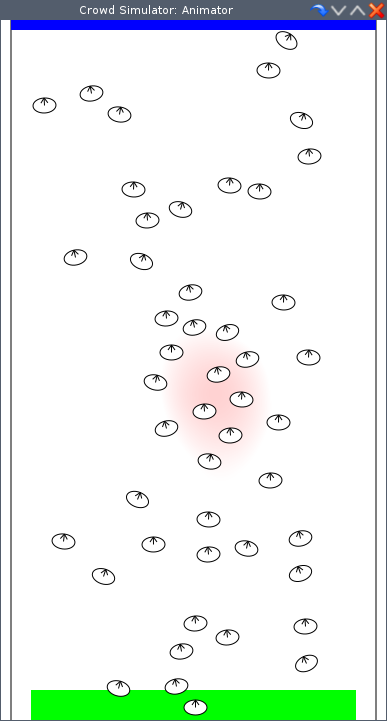
\includegraphics[scale=0.6]{screenshot}
  \caption{Снимок экрана модуля отображения результатов}
  \label{sec:manual:launch:scheenshot}
\end{figure}

Для запуска в режиме воспроизведения ранее записанного файла необходимо сначало сгенерировать файл командой
cat \$PATH\_TO\_SCENARIO \-|\- preprocessor/run.rb \-|\- core/target/release/core \->\- \$FILE\_WITH\_SIM\_RESULTS,
а затем запускать модуль отображения результатов командой \\
cat \$FILE\_WITH\_SIM\_RESULTS \-|\- animator/animator \\ animator/resources/person\_1.svg 1.0.

Также следует упомянуть возможность модуля отображения результатов использовать любую картинку в формате SVG в качестве текстуры пешехода.
Первым аргументом при запуске модуля указывается файл в формате SVG с картинкой пешехода (направление движения "--- вверх), а вторым "--- масштаб картинки в миллиметрах на пиксель.
Рекомендуется выбирать масштаб таким образом, чтобы итоговый размер пешехода был примерно равен 0.5 метра.

Пример результата работы ПС представлен на рисунке~\ref{sec:manual:launch:result_pic}.

\begin{figure}[ht]
  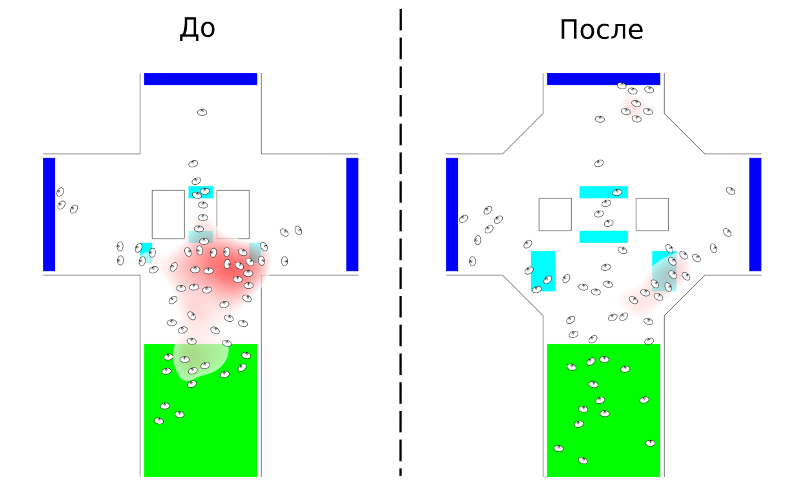
\includegraphics[width=\linewidth]{output_example}
  \caption{Пример результата работы ПС}
  \label{sec:manual:launch:result_pic}
\end{figure}


\sectioncentered*{Заключение}
\addcontentsline{toc}{section}{Заключение}

В рамках данной работы было разработано программное средство определения вероятных областей скопления людей в помещениях.
Для выполнения поставленное задачи разработанное программное средство использует имитационное моделирование.
Выбранной моделью является модель социальных сил.

Разработанное программное средство реализует модифицированную версию модели социальных сил.
В целом можно сказать, что данное программное средство успешно решает задачу определения вероятных областей скопления людей в помещениях.

Однако у разработанного программного средства есть и ряд недостатков.
К недостаткам можно отнести:
\begin{itemize}
  \item неполную поддержку формата SVG;
  \item отсутствие в моделировании сценария паники;
  \item отсутствие режима интерактивного просмотра результатов симуляции.
\end{itemize}

В дальнейшем разработанное программное средство будет развиваться с целью устранения описанных выше недостатков.



% Зачем: Изменение надписи для списка литературы
% Почему: Пункт 2.8.1 Требований по оформлению пояснительной записки.
\renewcommand{\bibsection}{\sectioncentered*{Cписок использованных источников}}
\addcontentsline{toc}{section}{Cписок использованных источников}

% Зачем: Печать списка литературы. База данных литературы - файл bibliography_database.bib
\bibliography{bibliography_database}


% \includepdf позволяет включить в результирующий pdf документ часть другого pdf документа, сделанного
% например не с помощью TeX. Бывает полезно, если какие-то диаграммны нарисованы, например, с помощью 
% Microoft Office и сохранены в pdf.
%\includepdf[pages={-}]{documents_list.pdf}

\end{document}
